\documentclass[12pt]{article}
\usepackage{amsmath}
\usepackage{graphicx,psfrag,epsf,float, bm, subcaption}
\graphicspath{C:/Users/Colin/Documents/GitHub/BB_data_analysis/paper/fig/}
\usepackage{enumerate}
\usepackage{natbib}
\bibliographystyle{asa}
\usepackage{url} % not crucial - just used below for the URL

% no longer require relative path to figs
\graphicspath{{fig/}}

\usepackage[x11names]{xcolor}
\usepackage{framed} % provides framed env., should be removed in final draft
\definecolor{shadecolor}{rgb}{1,.5,.5}

% math macros 

\newcommand{\ind}{\stackrel{ind.}{\sim}}
\newcommand{\op}{\operatorname}
\DeclareMathOperator*{\argmin}{arg\,min}
\newcommand{\myequation}{\begin{equation}}
\newcommand{\myendequation}{\end{equation}}
\let\[\myequation
       \let\]\myendequation


\pdfminorversion=4
% NOTE: To produce blinded version, replace "0" with "1" below.
\newcommand{\blind}{0}

% DON'T change margins - should be 1 inch all around.
\addtolength{\oddsidemargin}{-.5in}%
\addtolength{\evensidemargin}{-.5in}%
\addtolength{\textwidth}{1in}%
\addtolength{\textheight}{1.3in}%
\addtolength{\topmargin}{-.8in}%



\begin{document}

{
  \title{\bf A Hierarchical Model for Heterogenous Reliability Field Data}
  \author{Eric Mittman, Colin Lewis-Beck, and William Q. Meeker\\
  Department of Statistics\\
  Iowa State University\\
  Ames, Iowa}
  \maketitle
} 

\def\spacingset#1{\renewcommand{\baselinestretch}%
{#1}\small\normalsize} \spacingset{1}

\begin{center}
{\large\bf SUPPLEMENTARY MATERIAL}
\end{center}

\newpage

{\appendix
\section{Truncation adjusted Kaplan-Meier estimate of lifetime}
\label{sec:trunc-adj}
We first start with a nonparametric estimate of the empirical cdf for each sub-population using the Kaplan-Meier estimator.  With left truncation, however, the standard Kaplan-Meier estimator for drive-model $g$, denoted by
$\widehat{F_g(t)}_{KM}$, is conditional on survival up to
$t_{g,\text{min}}^L$, the shortest reported running time of all units in
of sub-population $g$ for which records are available. To produce
unconditional estimates, we adapt the adjustment method outlined by \citet[Chapter 11]{meeker}.  For each sub-population we select
$t_{g,\text{min}}^L$, the smallest left truncated time in the sample.
By sampling from the full posterior distribution, because
$\Pr(T>t_{g,\text{min}}^L|\theta_g)$ (the probability that a hard drive has
survived up to $t_{g,\text{min}}^L$) is a function of the model
parameters, we can easily compute its posterior median,
$\widehat{A}_{\text{med}} = \widehat{\Pr}(T>t_{g,\text{min}}^L|\theta_g)$. We compute the adjusted estimate by

$$\widehat{F(t)}_{KMadj} = \widehat{A}_{\text{med}} + \left(1 - \widehat{A}_{\text{med}}\right)\widehat{F_g(t)}_{KM},\; t>t_{g,\text{min}}^L.$$

While this adjustment may be negligible for sub-populations with little truncation, in our Backblaze example, five drive-models receive upward adjustments of greater than 5 percent and the estimated time to failure distribution of one drive-model (30) was adjusted by nearly 16 percent, in part because the shortest truncation time for all observed units was approx. 2.3 years.

\section{Definition of global average for Model 4}
\label{global-avg}
In Section 7, to illustrate the concept of shrinkage in our hierarchical model, we refer to a ``global average" which represents an average GLFP cdf for the entire population, $\op{H}\left(\cdot|\bar{\pi},\mu_1,\sigma_1,\bar{\mu}_2,\bar{\sigma}_2\right)$. Because $\mu_1$ and $\sigma_1$ are common across all sub-populations in our model, these can already be interpreted as ``global." For the parameters that vary across sub-populations, we select values corresponding to the medians of the hierarchical distributions (4) conditional on the hyperparameters. In particular, we set
$$\bar{\pi}=\op{logit}^{-1}(\eta_{\pi}),\;\bar{\mu}_2=\eta_{t_2} - m_{\sigma_2}\Phi^{-1}(.2) \mbox{ and } \bar{\sigma}_2= m_{\sigma_2}.$$
Let $J(\cdot|a,b),\;J^{-1}(\cdot|a,b)$ denote the cdf and inverse cdf, respectively, for a lognormal distribution with log-location parameter $a$ and log-scale parameter $b$. Then
$$m_{\sigma_2}=J^{-1}[0.5 \cdot J(1|\eta_{\sigma_2},\tau_{\sigma_2})|\eta_{\sigma_2}, \tau_{\sigma_2}],$$
which is the median of a lognormal distribution with parameters $\eta_{\sigma_2}$, and $\tau_{\sigma_2}$, truncated to the interval $(0, 1)$.

We estimate the global average pointwise, using draws from the joint posterior distribution, $H\left(\tilde{t}|\eta_\pi^{(s)}, \mu_1^{(s)}, \sigma_1^{(s)}, \eta_{t_2}^{(s)},\eta_{\sigma_2}^{(s)},\tau_{\sigma_2}^{(s)}\right)$, $s=1,2,\ldots,S$. The computation is thus similar to that shown in (7).
}

%\begin{description}

%\item Stan code for Model 4, estimated using the Backblaze data set (also available as a supplementary .csv file).

%\end{description}

\section{Stan code for Model 4}
\label{sec:stan-code}
{\scriptsize
\begin{verbatim}
functions {
real sev_logpdf(real y, real mu, real sigma){
real z;
z = (y - mu) / sigma;
return -log(sigma) + z - exp(z);
}

real sev_logccdf(real y, real mu, real sigma){
return -exp((y - mu) / sigma);
}

real sev_logcdf(real y, real mu, real sigma){
return log1m_exp(-exp((y - mu) / sigma));
}
}

data {
int M;
int N_obs;
int N_cens;
real endtime_obs[N_obs];
real endtime_cens[N_cens];
real starttime_obs[N_obs];
real starttime_cens[N_cens];
int<lower=1, upper=M> dm_obs[N_obs];
int<lower=1, upper=M> dm_cens[N_cens];
vector<lower=0, upper=1>[2] p; # quantiles to model
}
transformed data{
vector[2] z_corr;
for(i in 1:2)
z_corr[i] = log(-1.0 * log1m(p[i])); # used to get location(mu) from quantile(t_p)
}
parameters{
real log_tp1;
real<lower=0> sigma1;
real eta_tp2;
real eta_s2;
real eta_pi;
real<lower=0> tau_tp2;
real<lower=0> tau_s2;
real<lower=0> tau_pi;
vector[M] log_tp2_raw;
real<lower=0, upper=1> sigma2[M];
vector[M] logit_pi_raw;
}

transformed parameters{
real mu1;
vector[M] mu2;
vector[M] log_pi;
mu1 = log_tp1 - sigma1 * z_corr[1];
for(m in 1:M){
mu2[m] = (eta_tp2 + tau_tp2 * log_tp2_raw[m]) - (sigma2[m] * z_corr[2]);
}
for(m in 1:M)
log_pi[m] = log_inv_logit(eta_pi + tau_pi * logit_pi_raw[m]);
}

model{
real tmp[2];
int m;
real logpi;
real mu_1;
real mu_2;
real sig_1;
real sig_2;

for(i in 1:N_obs){
m = dm_obs[i];
logpi = log_pi[m];
mu_2 = mu2[m];
sig_2 = sigma2[m];
// numerator:   log( p * f1 * (1 - F2) + f2 * (1 - p * F1) )
//            = log( exp(log(p) + log(f1) + log(1 - F2)) + exp(log(f2) + log(1 - exp(log(p) + log(F1)))) )
tmp[1] = log_sum_exp(logpi + sev_logpdf(endtime_obs[i], mu1, sigma1) +
sev_logccdf(endtime_obs[i], mu_2, sig_2),
sev_logpdf( endtime_obs[i], mu_2, sig_2) +
log1m_exp(logpi + sev_logcdf(endtime_obs[i], mu1, sigma1)
)
);
// denominator:  log((1 - p * F1) * (1 - F2))
//            =  log(1 - p * F1) + log(1 - F2)
tmp[2] = log1m_exp(logpi + sev_logcdf(starttime_obs[i], mu1, sigma1)) +
sev_logccdf(starttime_obs[i], mu_2, sig_2);

target += tmp[1] - tmp[2];
}

for(i in 1:N_cens){
m = dm_cens[i];
logpi = log_pi[m];
mu_2 = mu2[m];
sig_2 = sigma2[m];

// numerator:   log((1 - p * F1) * (1 - F2))
//            =  log(1 - p * F1) + log(1 - F2)
tmp[1] = log1m_exp(logpi + sev_logcdf(endtime_cens[i], mu1, sigma1)) +
sev_logccdf(endtime_cens[i], mu_2, sig_2);
// denominator:  log((1 - p * F1) * (1 - F2))
//            =  log(1 - p * F1) + log(1 - F2)
tmp[2] = log1m_exp(logpi + sev_logcdf(starttime_cens[i], mu1, sigma1)) +
sev_logccdf(starttime_cens[i], mu_2, sig_2);

target += tmp[1] - tmp[2];
}

log_tp1        ~ normal(7, 2);
log_tp2_raw    ~ normal(0, 1);
sigma1         ~ lognormal(0, 1);
sigma2         ~ lognormal(eta_s2, tau_s2);
logit_pi_raw   ~ normal(0, 1);
eta_tp2        ~ normal(9, 2);
eta_s2         ~ normal(0, 2);
eta_pi         ~ normal(-3, 1);
tau_tp2        ~ cauchy(0,1);
tau_s2         ~ cauchy(0,1);
tau_pi         ~ cauchy(0,1);
}

\end{verbatim}
}

\pagebreak
\section{Posterior predictive graphical checks}
Full set of Figures 5 and 6 for all 44 drive-models.  Numbering in the top left indicates drive-model.  Left: Adjusted K-M estimates of the proportion failing.  The original data (bold line) and 19 ``replicated" data sets from the posterior predictive distribution (dashed lines) are shown.  Right: Posterior median of proportion failing as a function of time for Models 1-4.  Plotted on Weibull probability scales.  The solid step function is the adjusted K-M estimate.  
\begin{figure}[H]
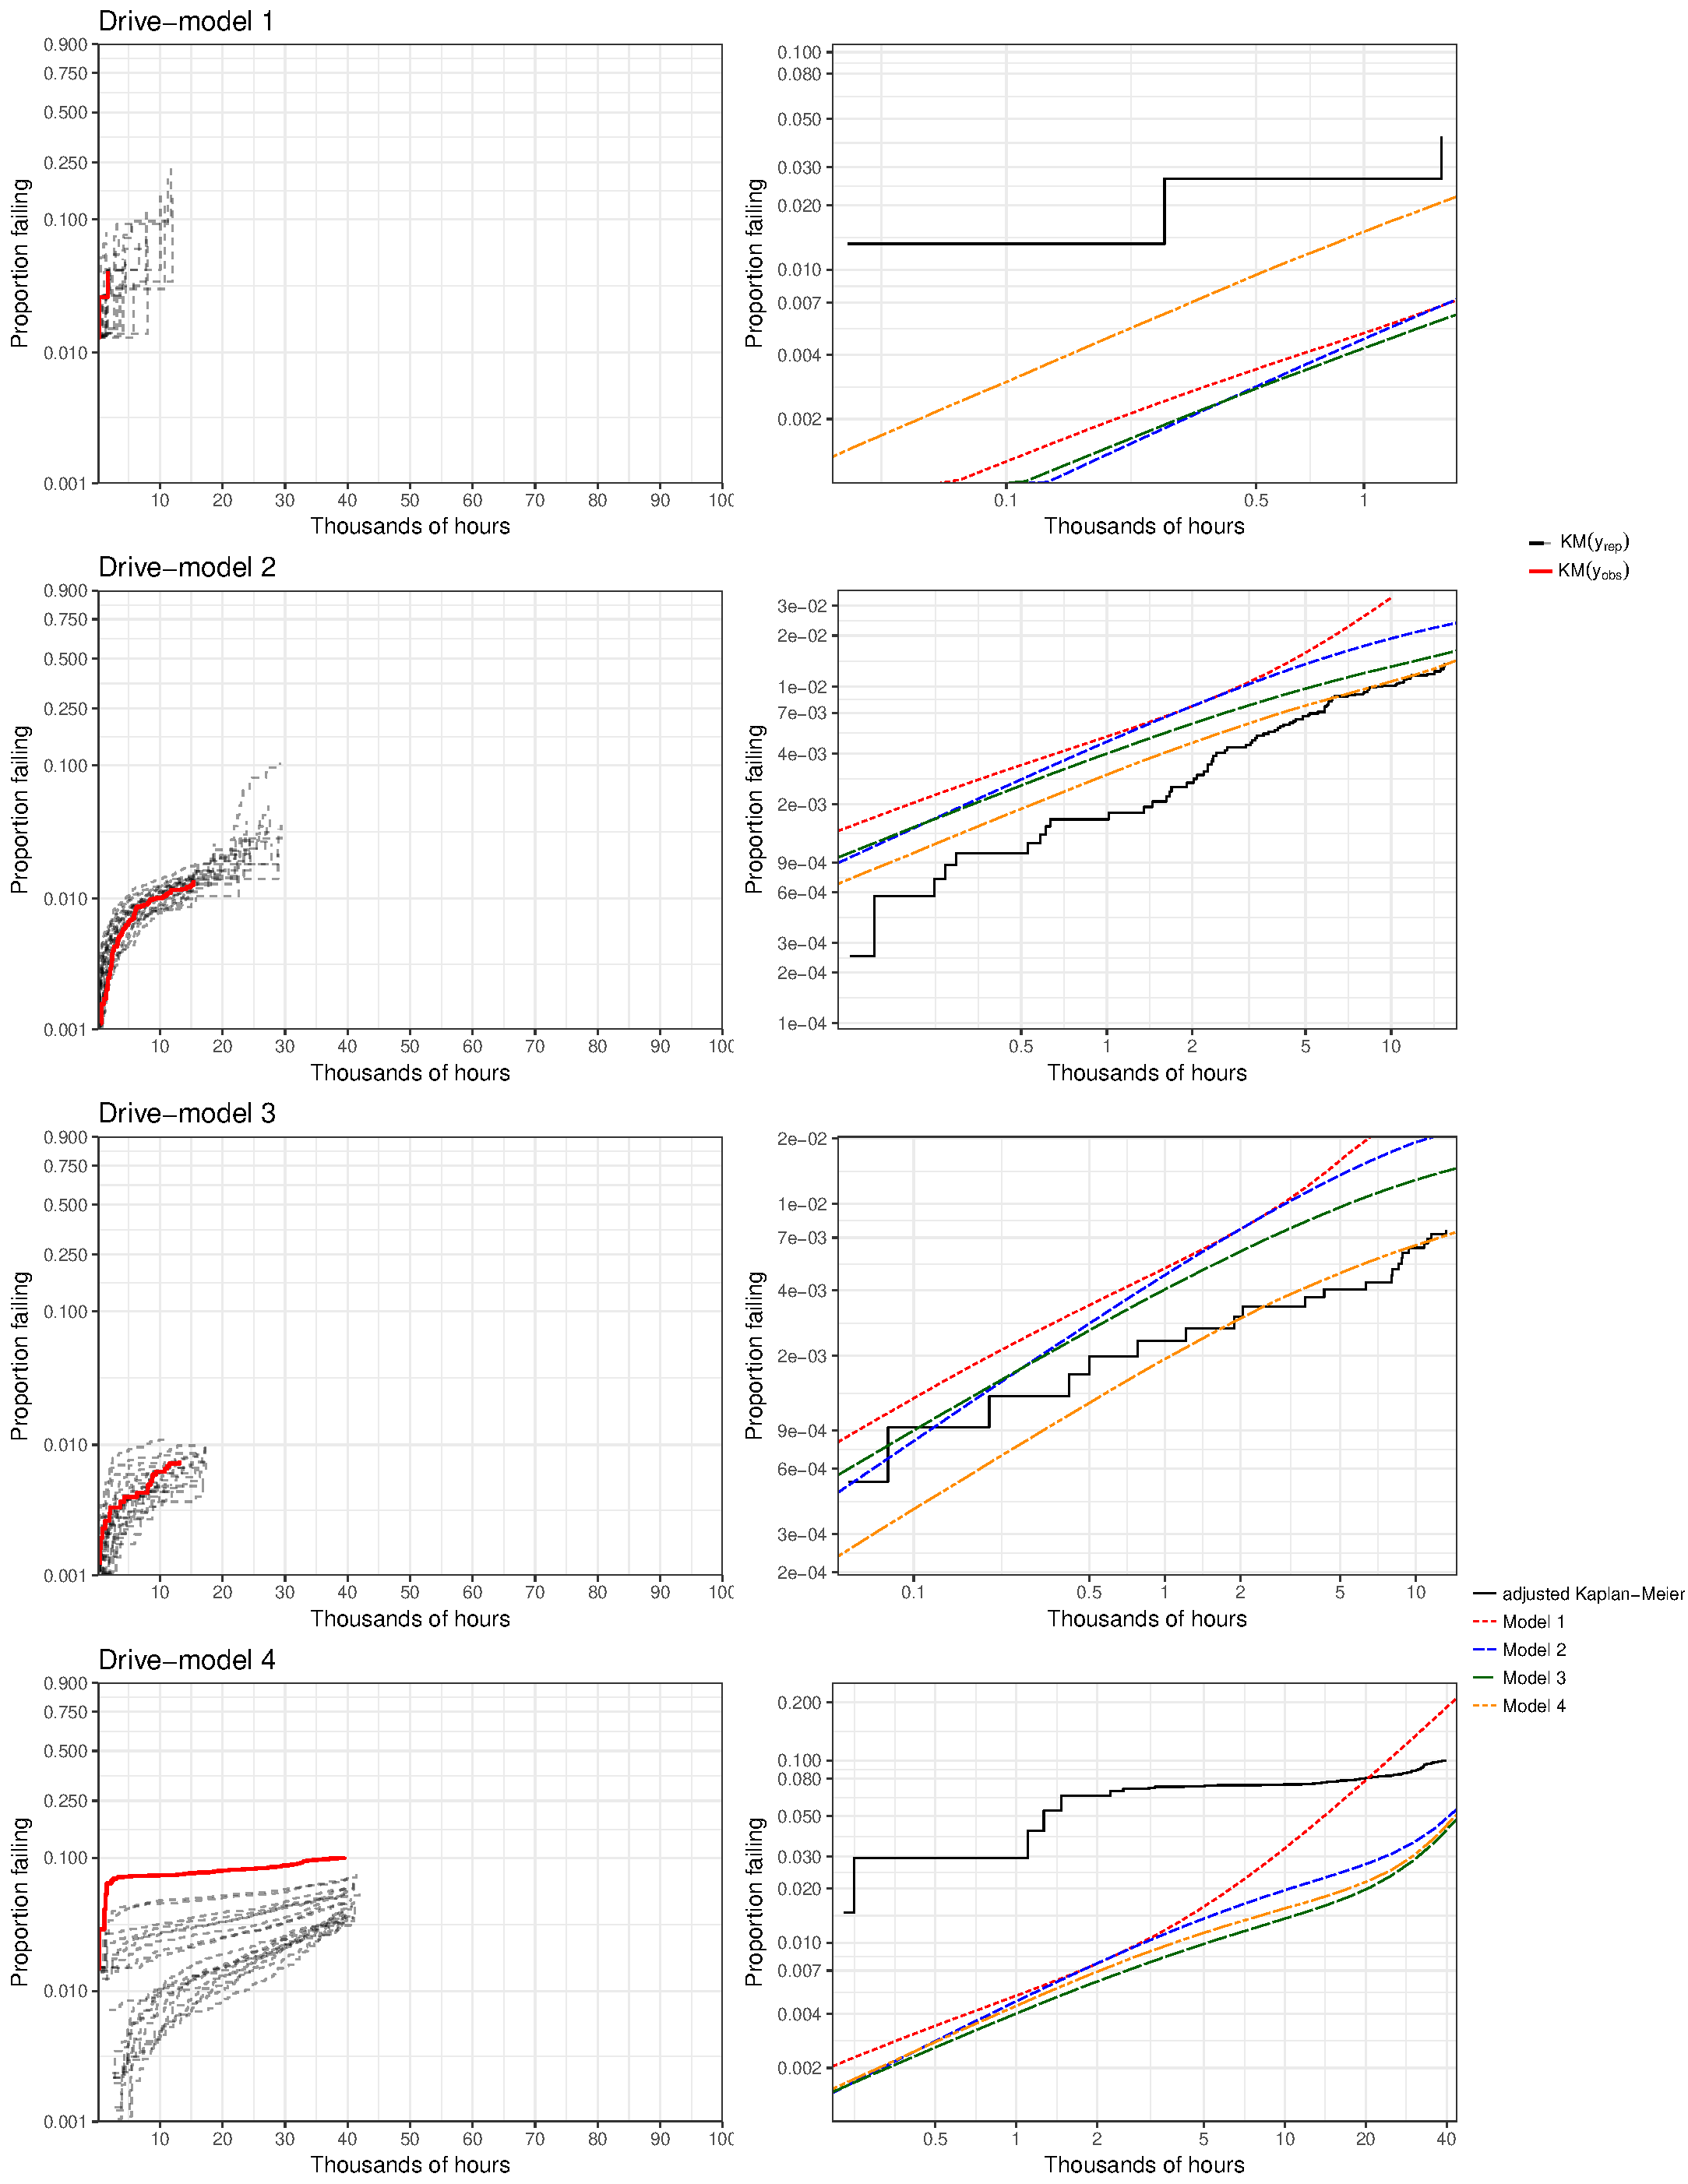
\includegraphics[width=\textwidth]{ppcheck-v3-1.pdf}
\end{figure}
\begin{figure}[H]
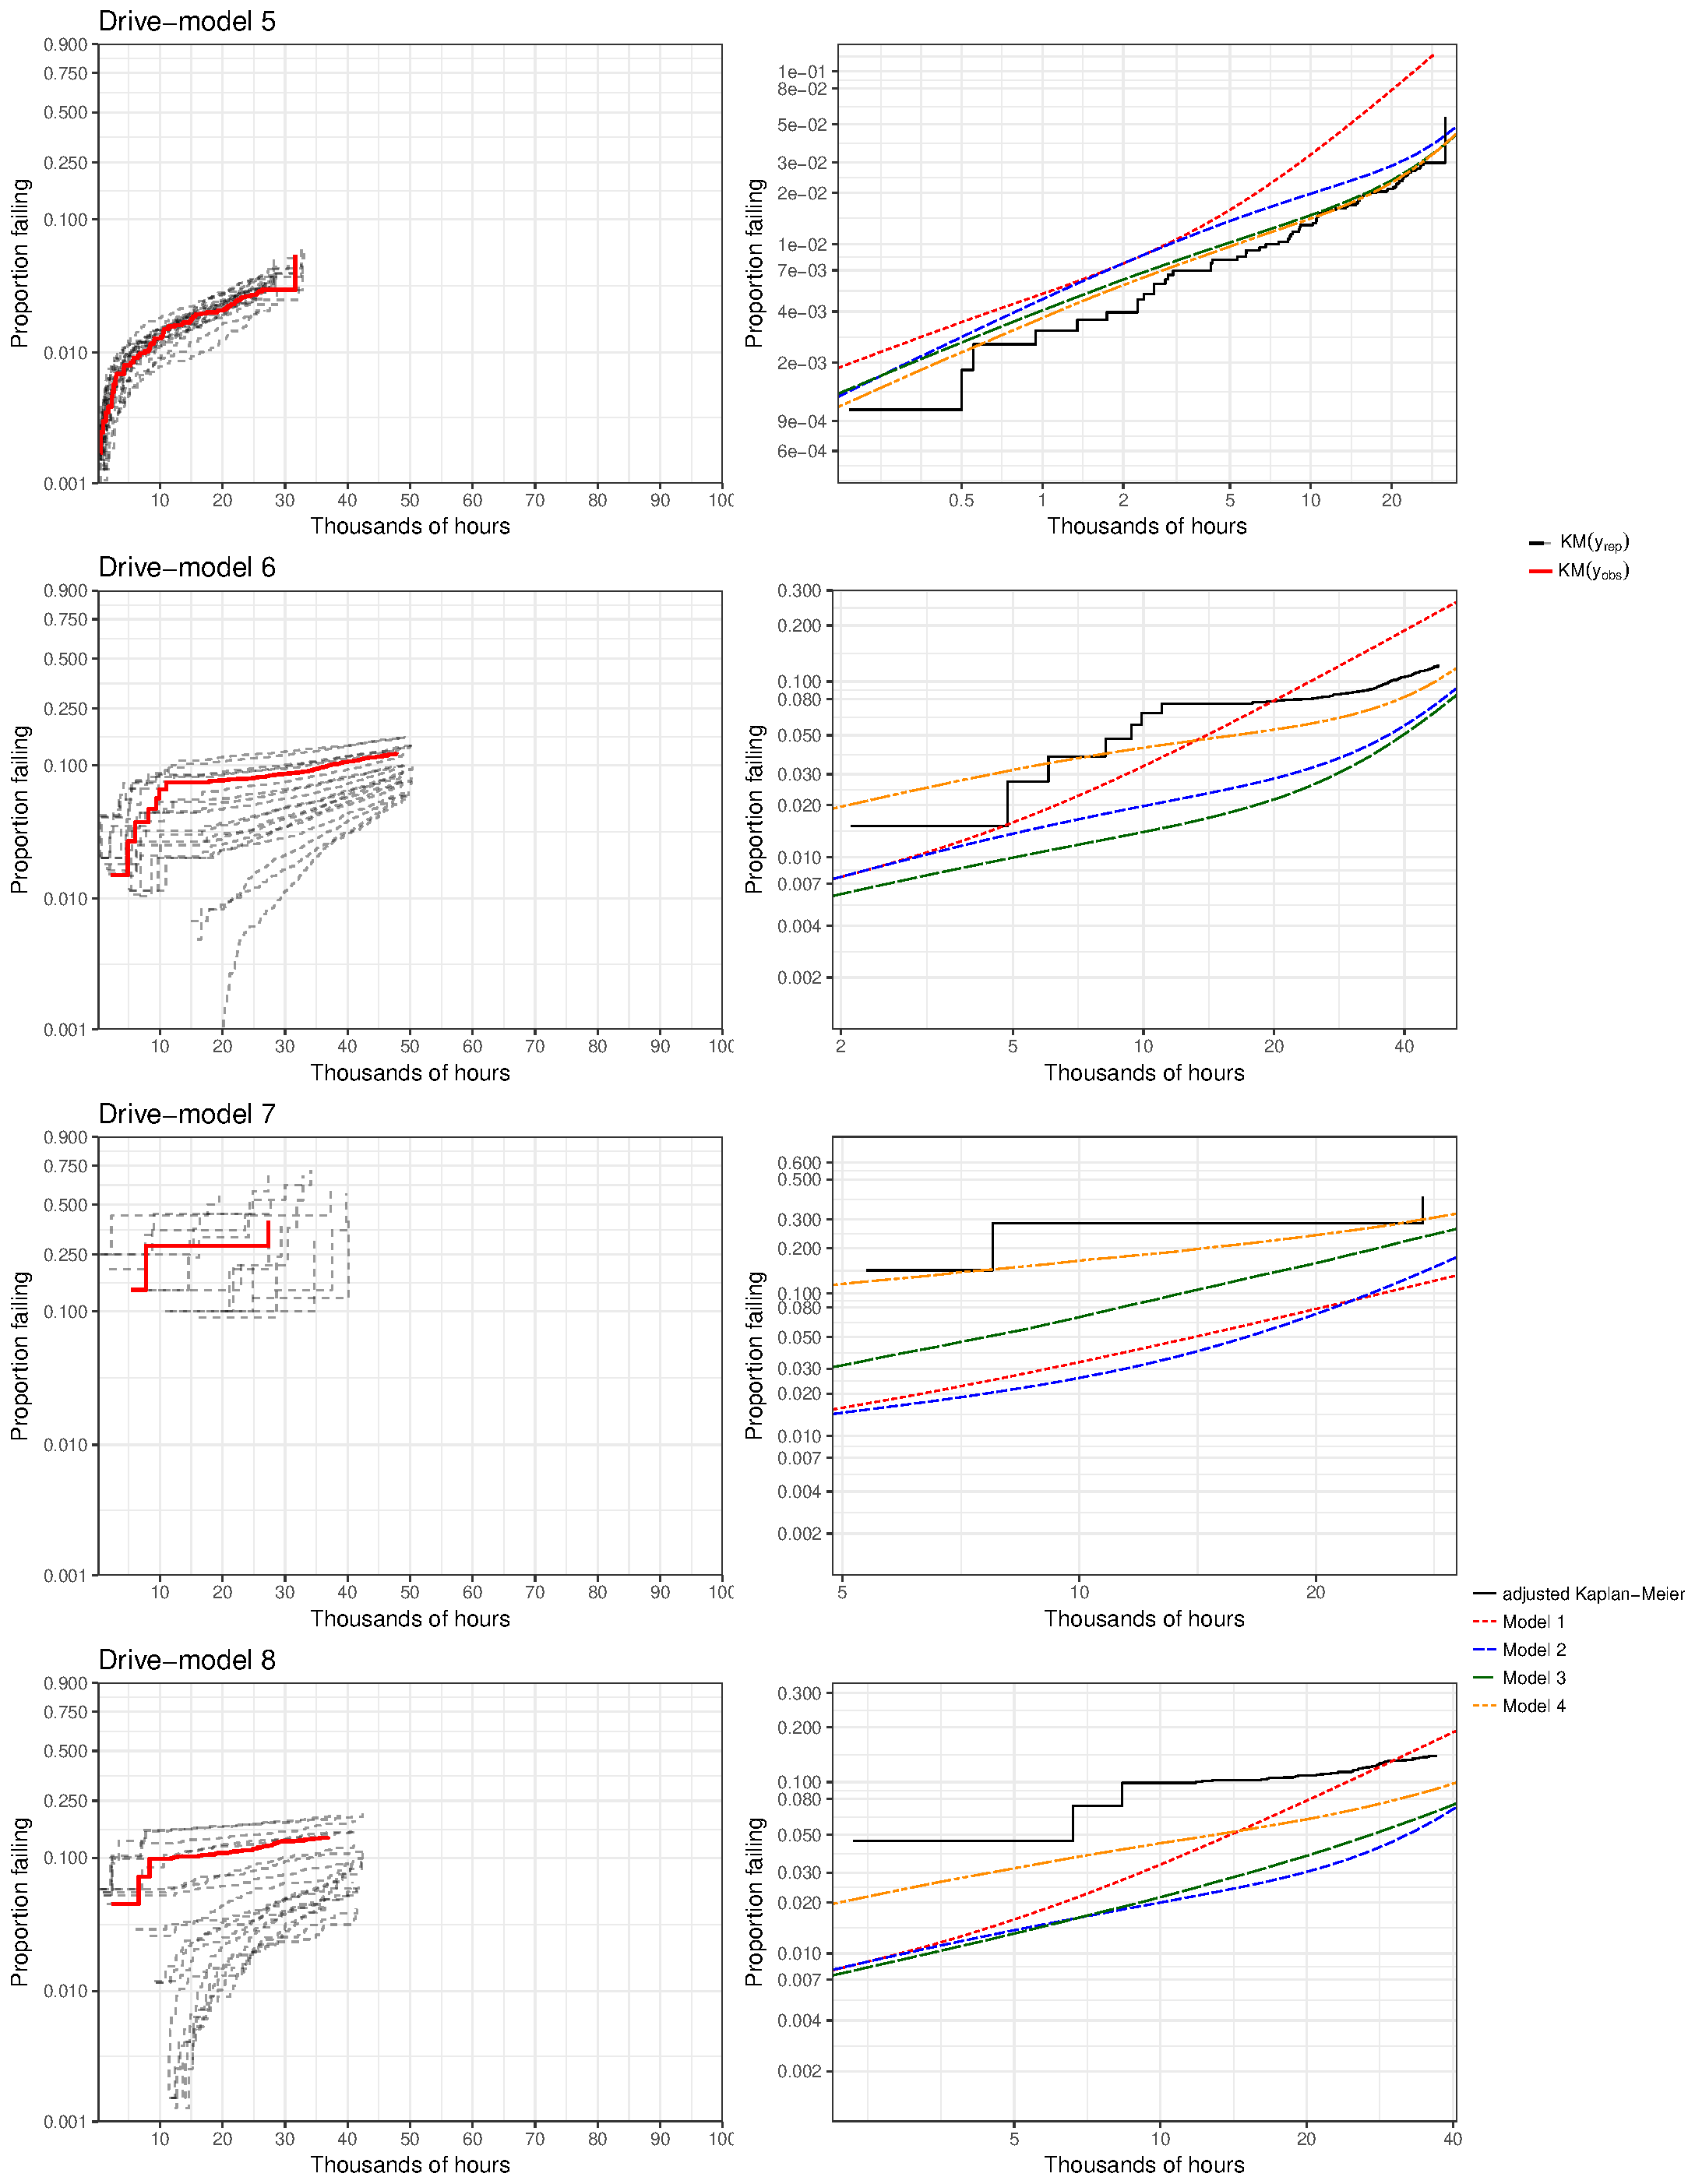
\includegraphics[width=\textwidth]{ppcheck-v3-2}
\end{figure}
\begin{figure}[H]
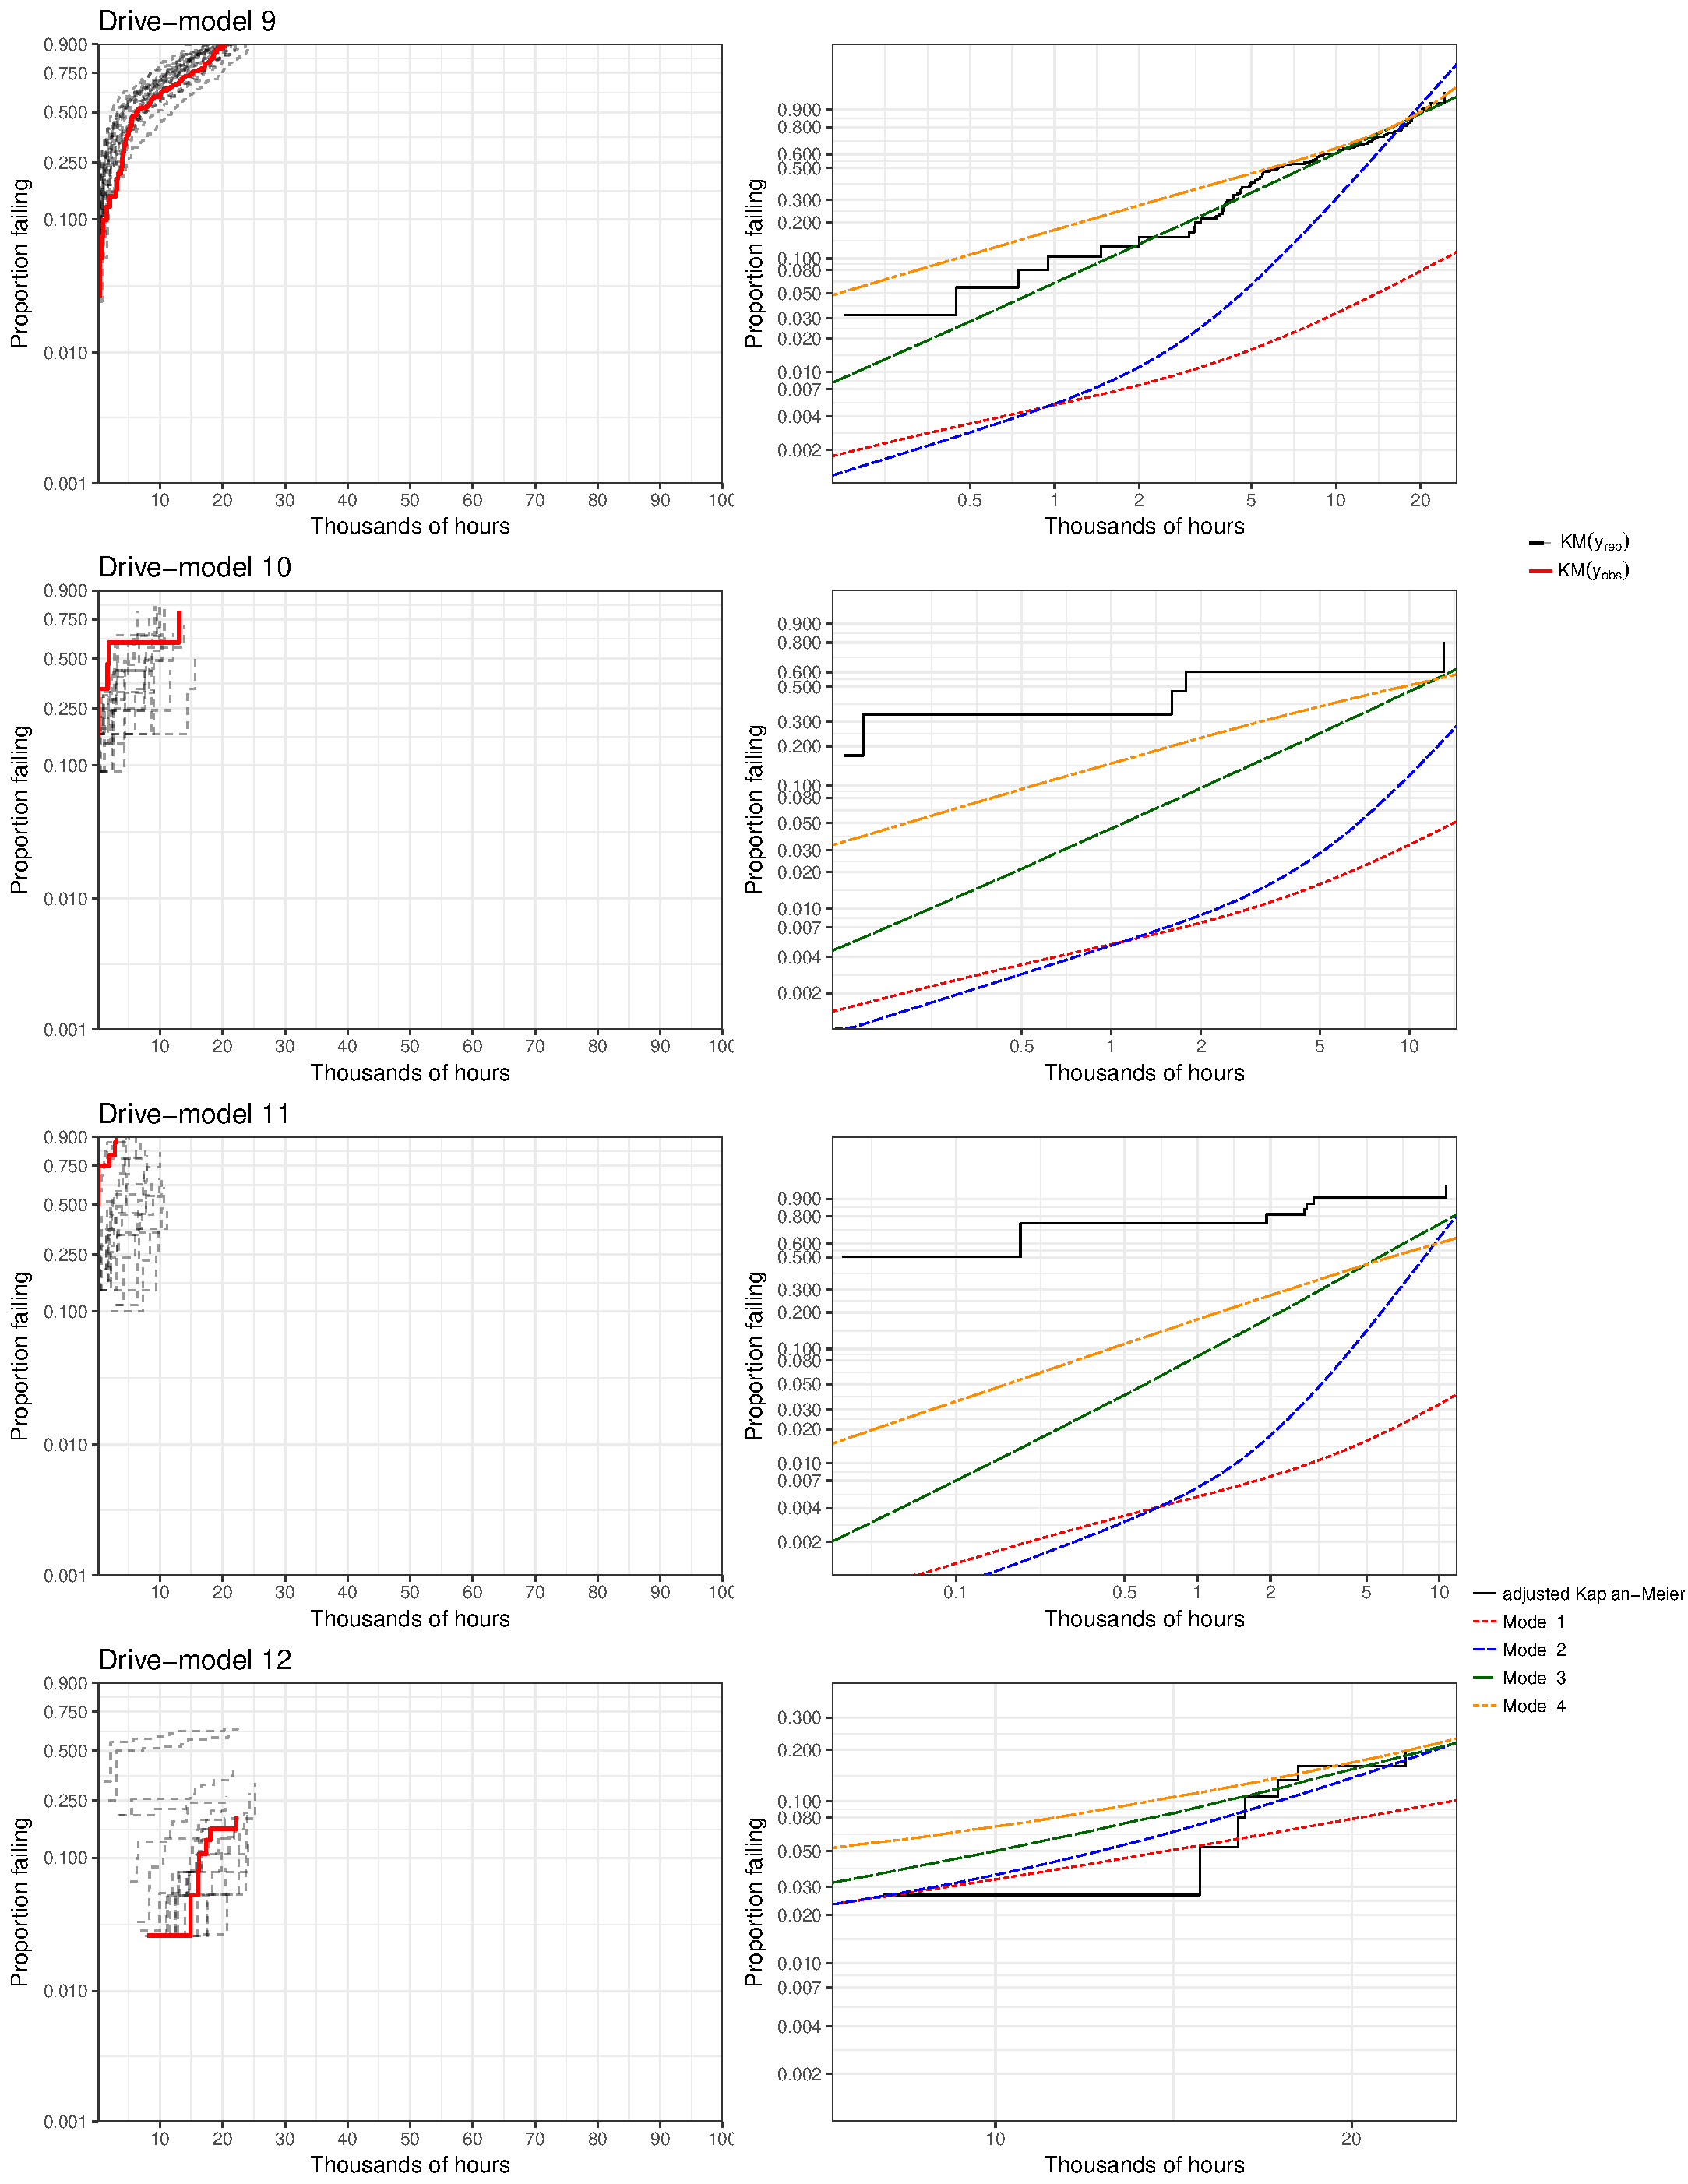
\includegraphics[width=\textwidth]{ppcheck-v3-3.pdf}
\end{figure}
\begin{figure}[H]
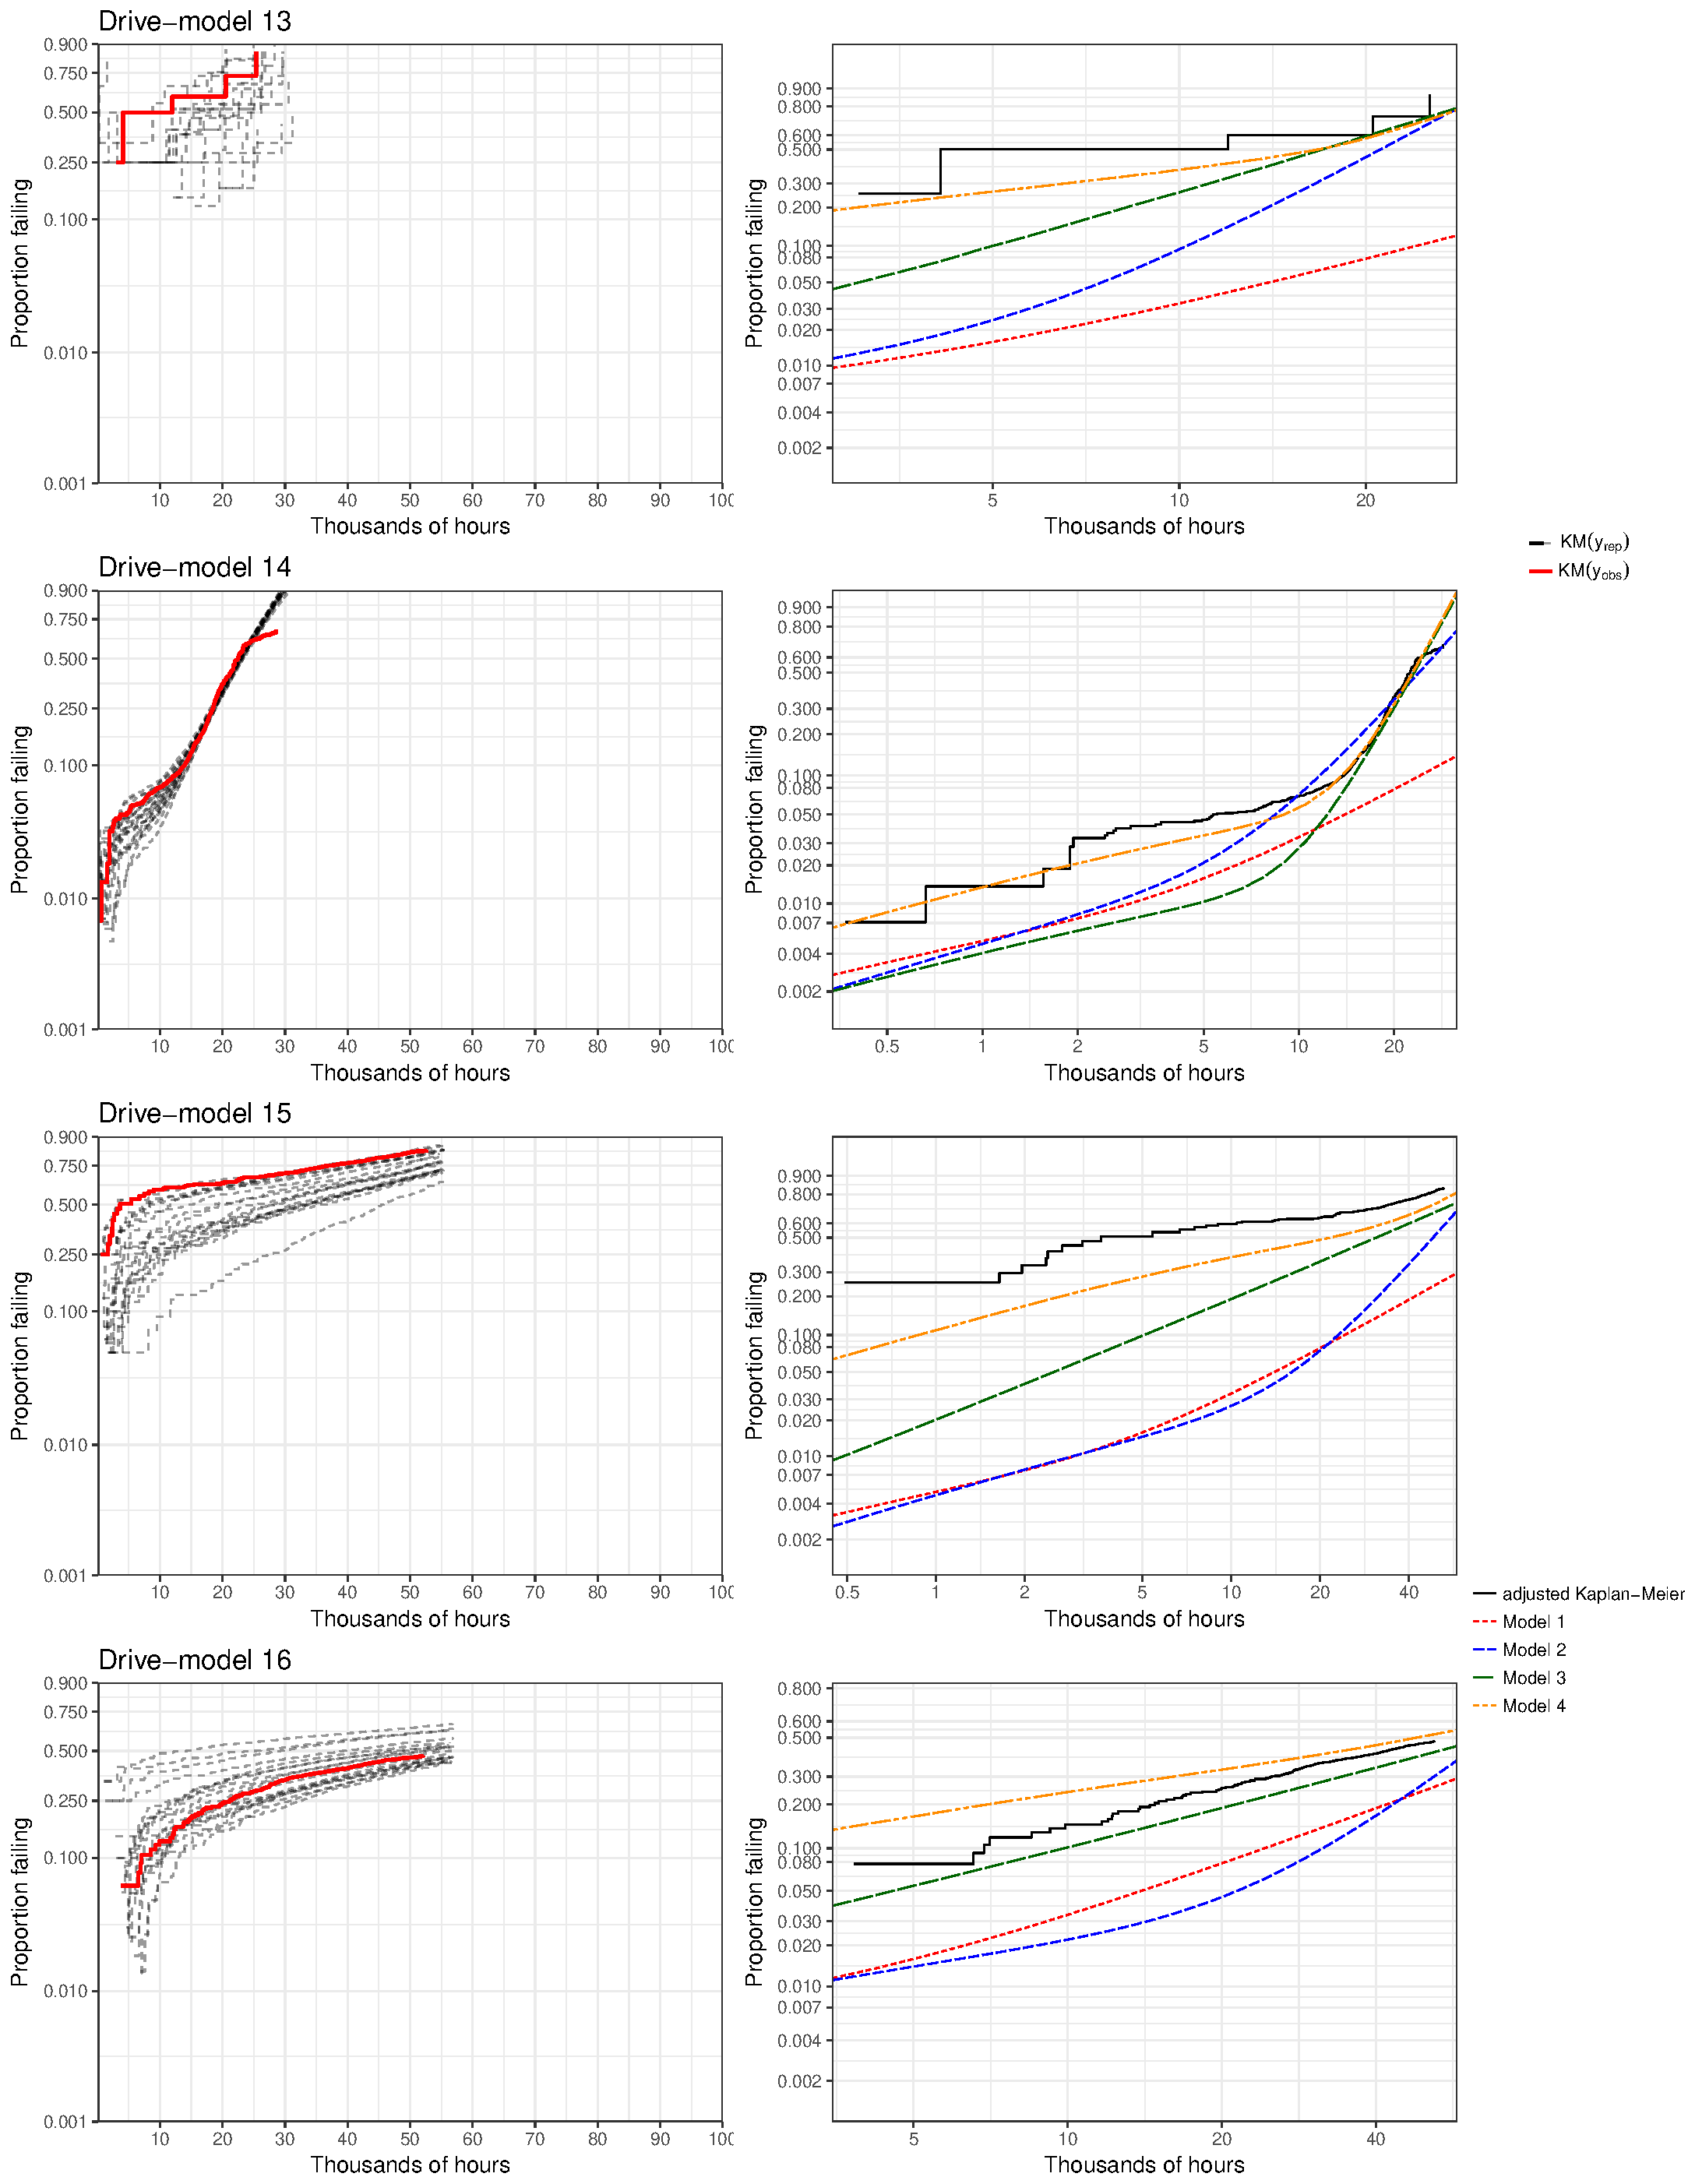
\includegraphics[width=\textwidth]{ppcheck-v3-4.pdf}
\end{figure}
\begin{figure}[H]
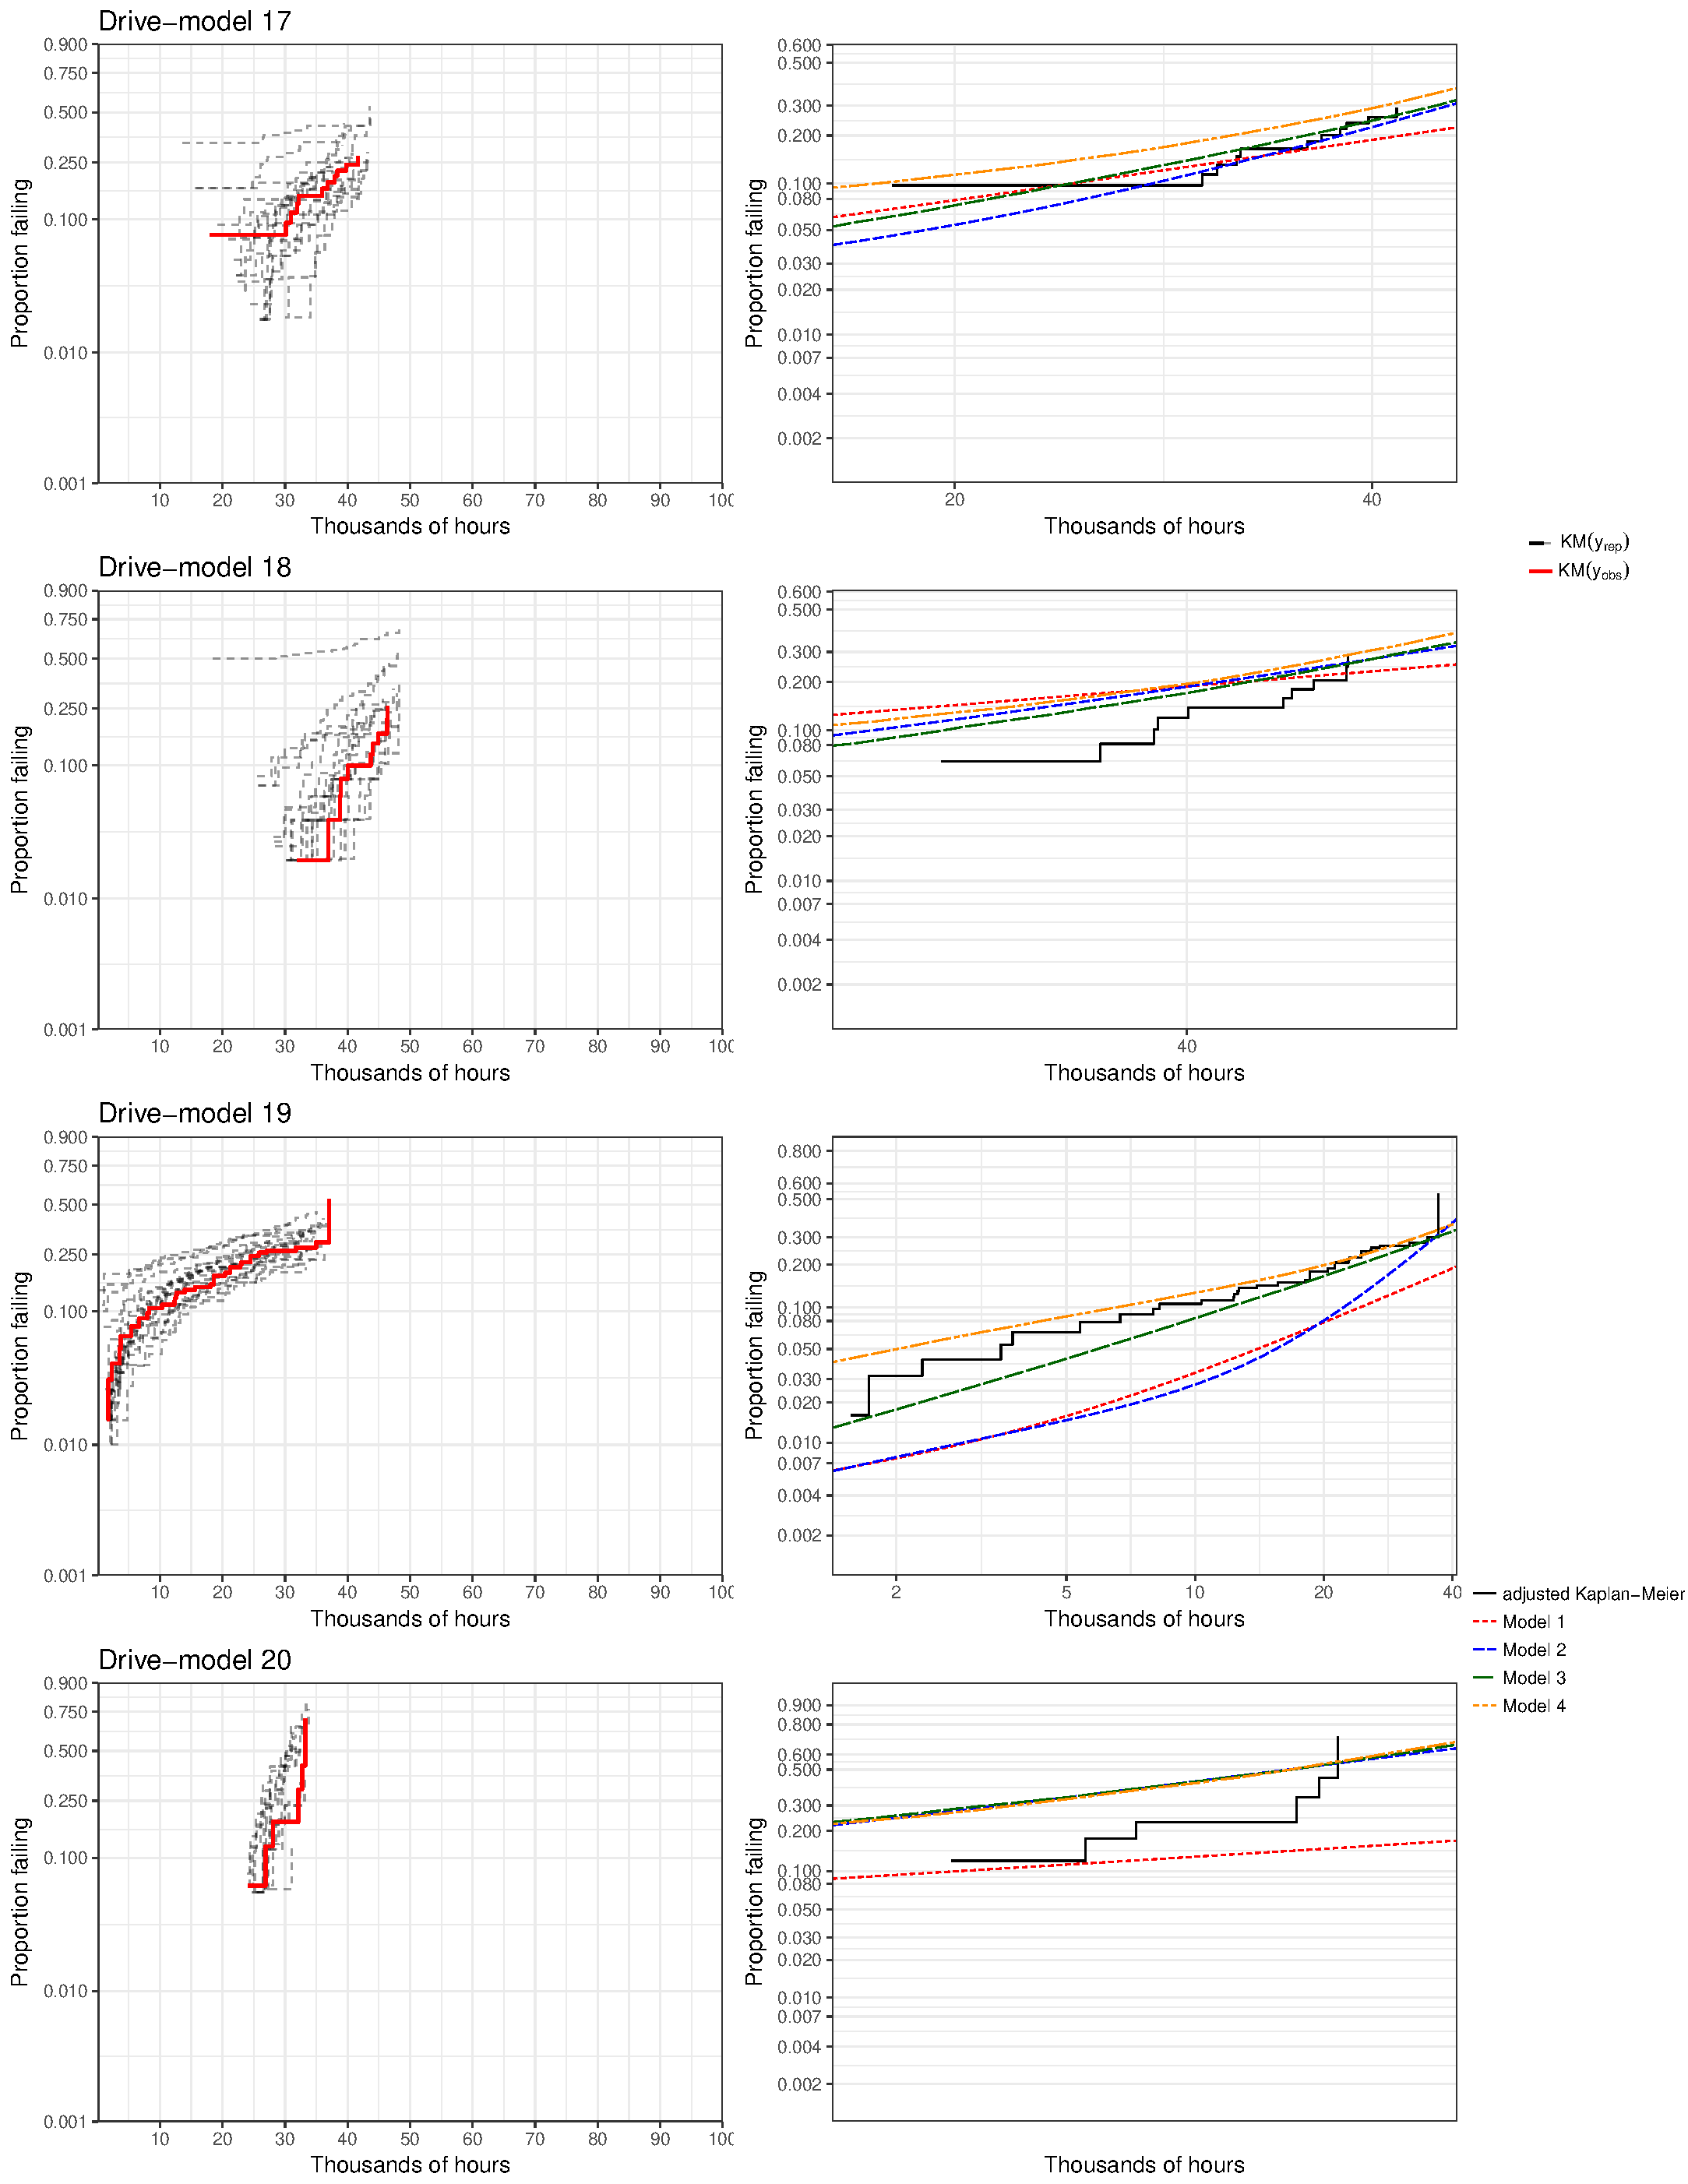
\includegraphics[width=\textwidth]{ppcheck-v3-5.pdf}
\end{figure}
\begin{figure}[H]
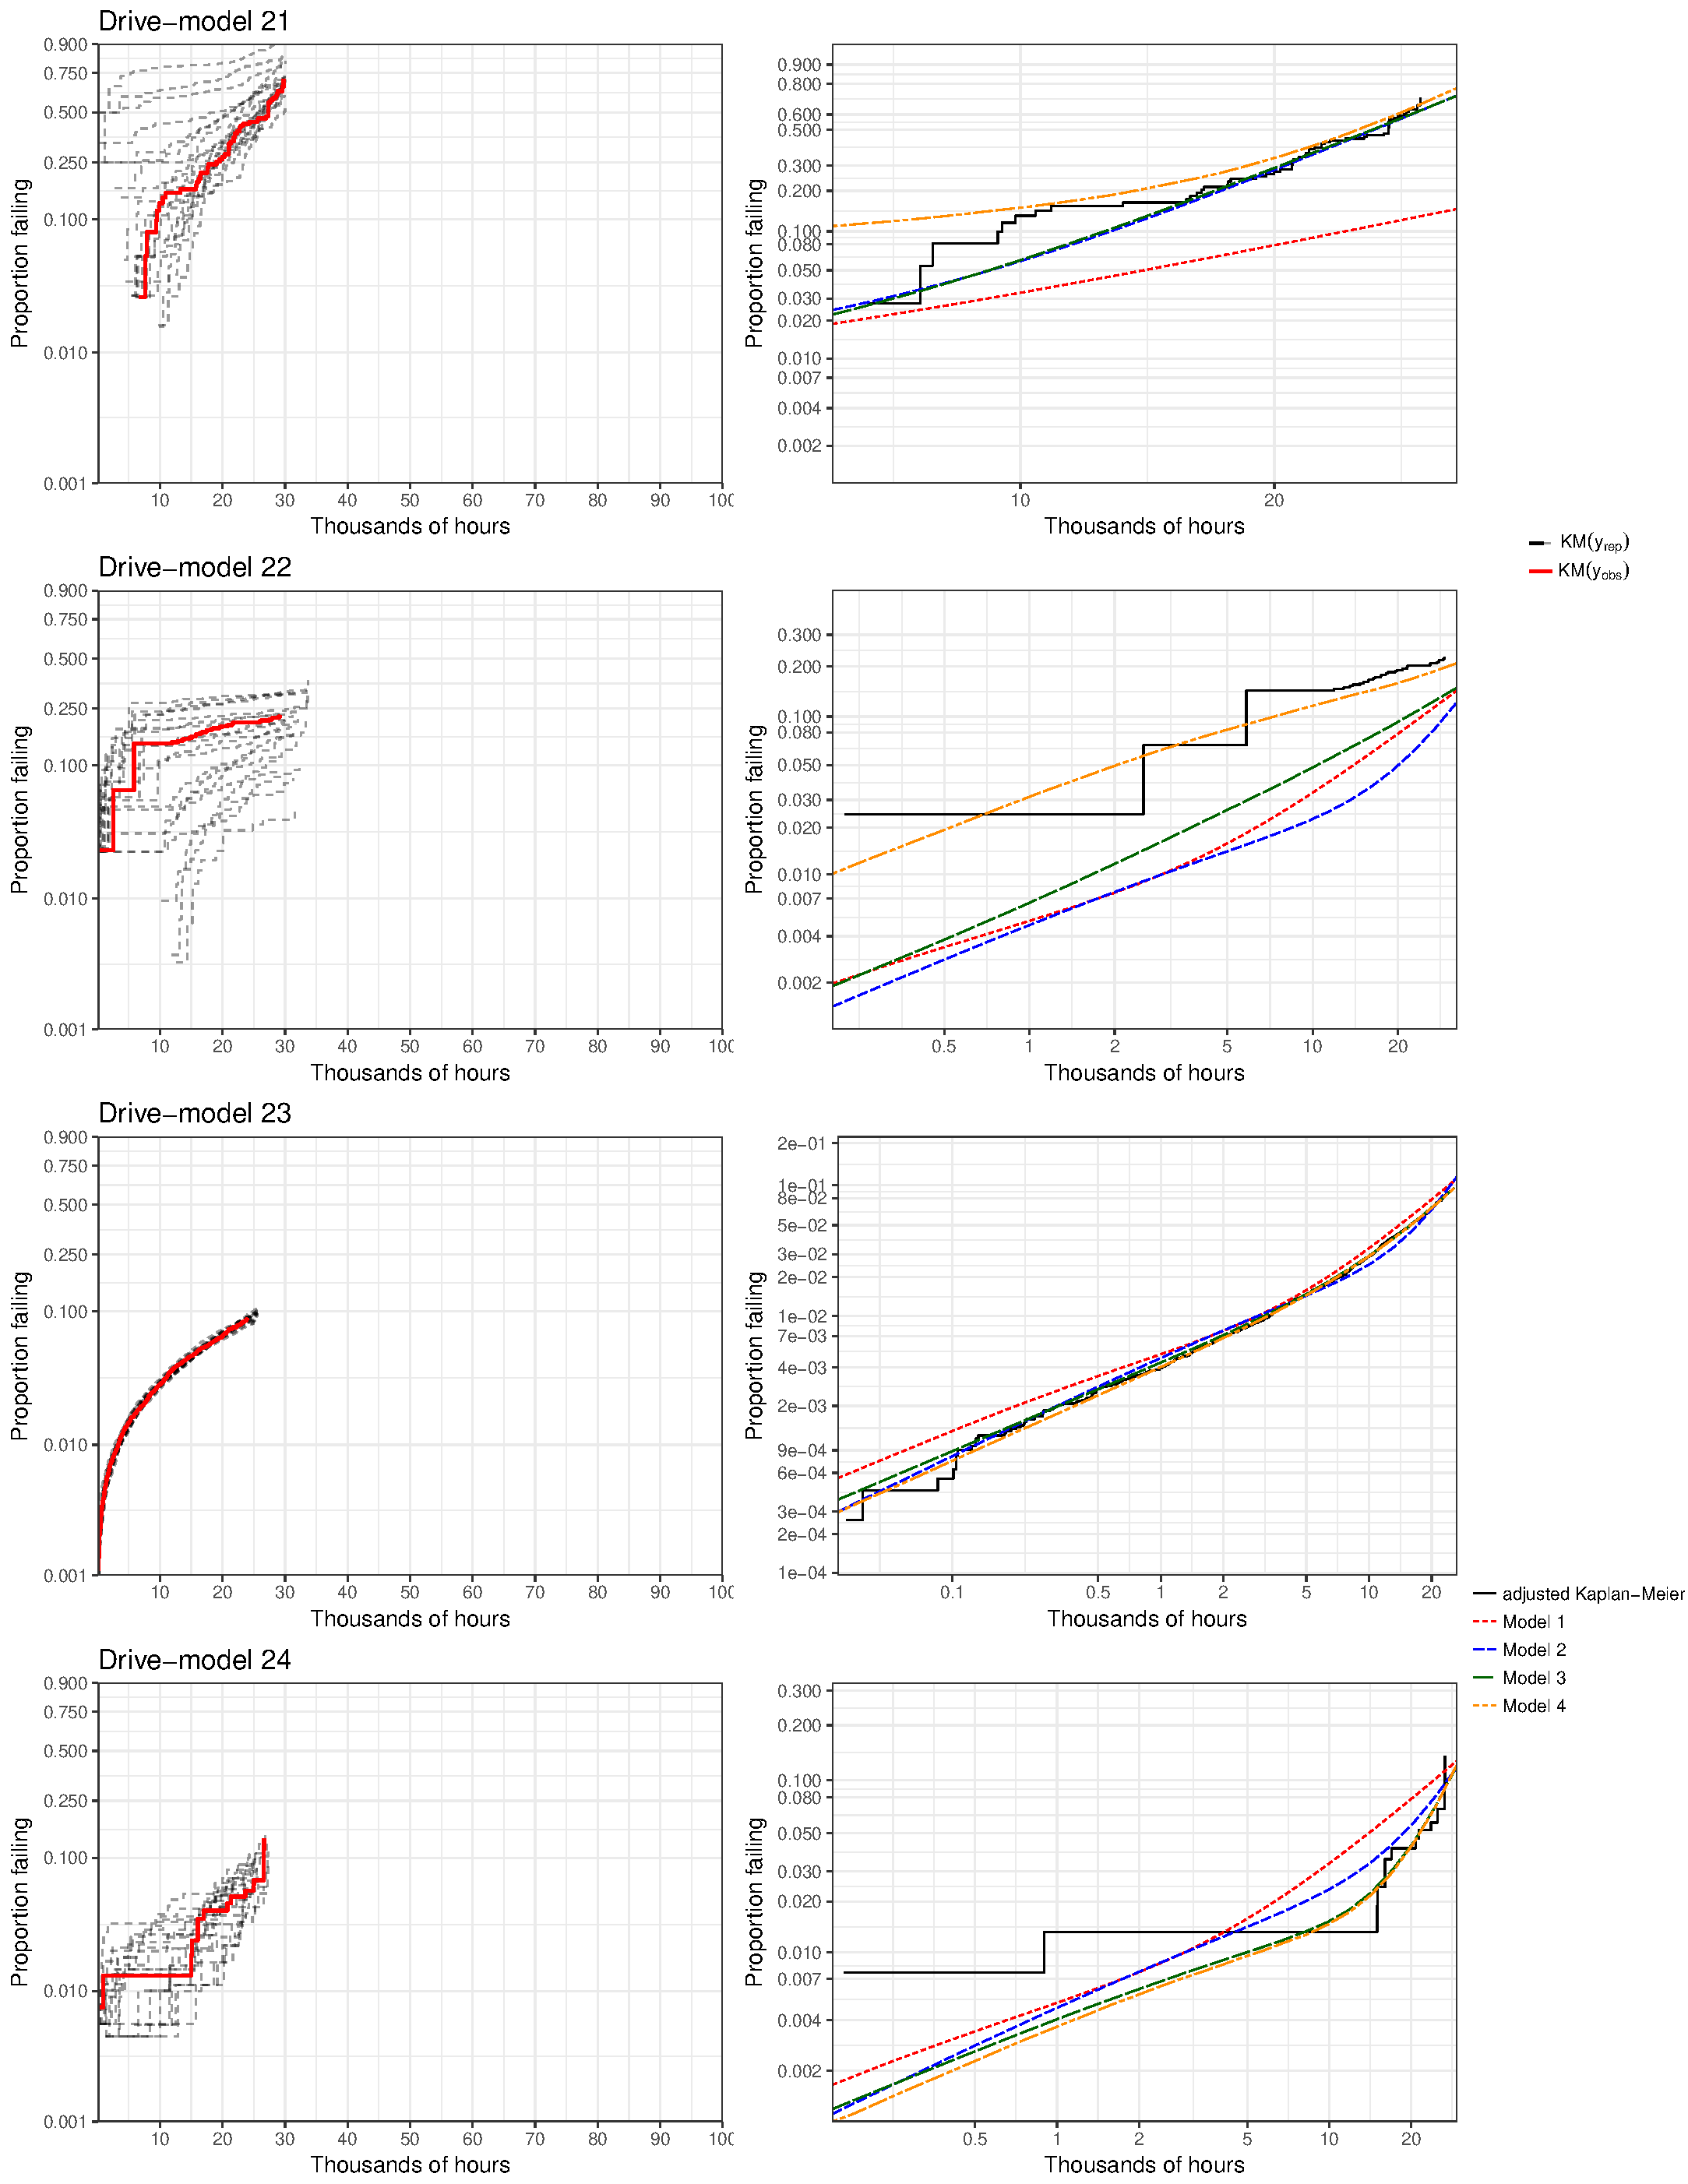
\includegraphics[width=\textwidth]{ppcheck-v3-6.pdf}
\end{figure}
\begin{figure}[H]
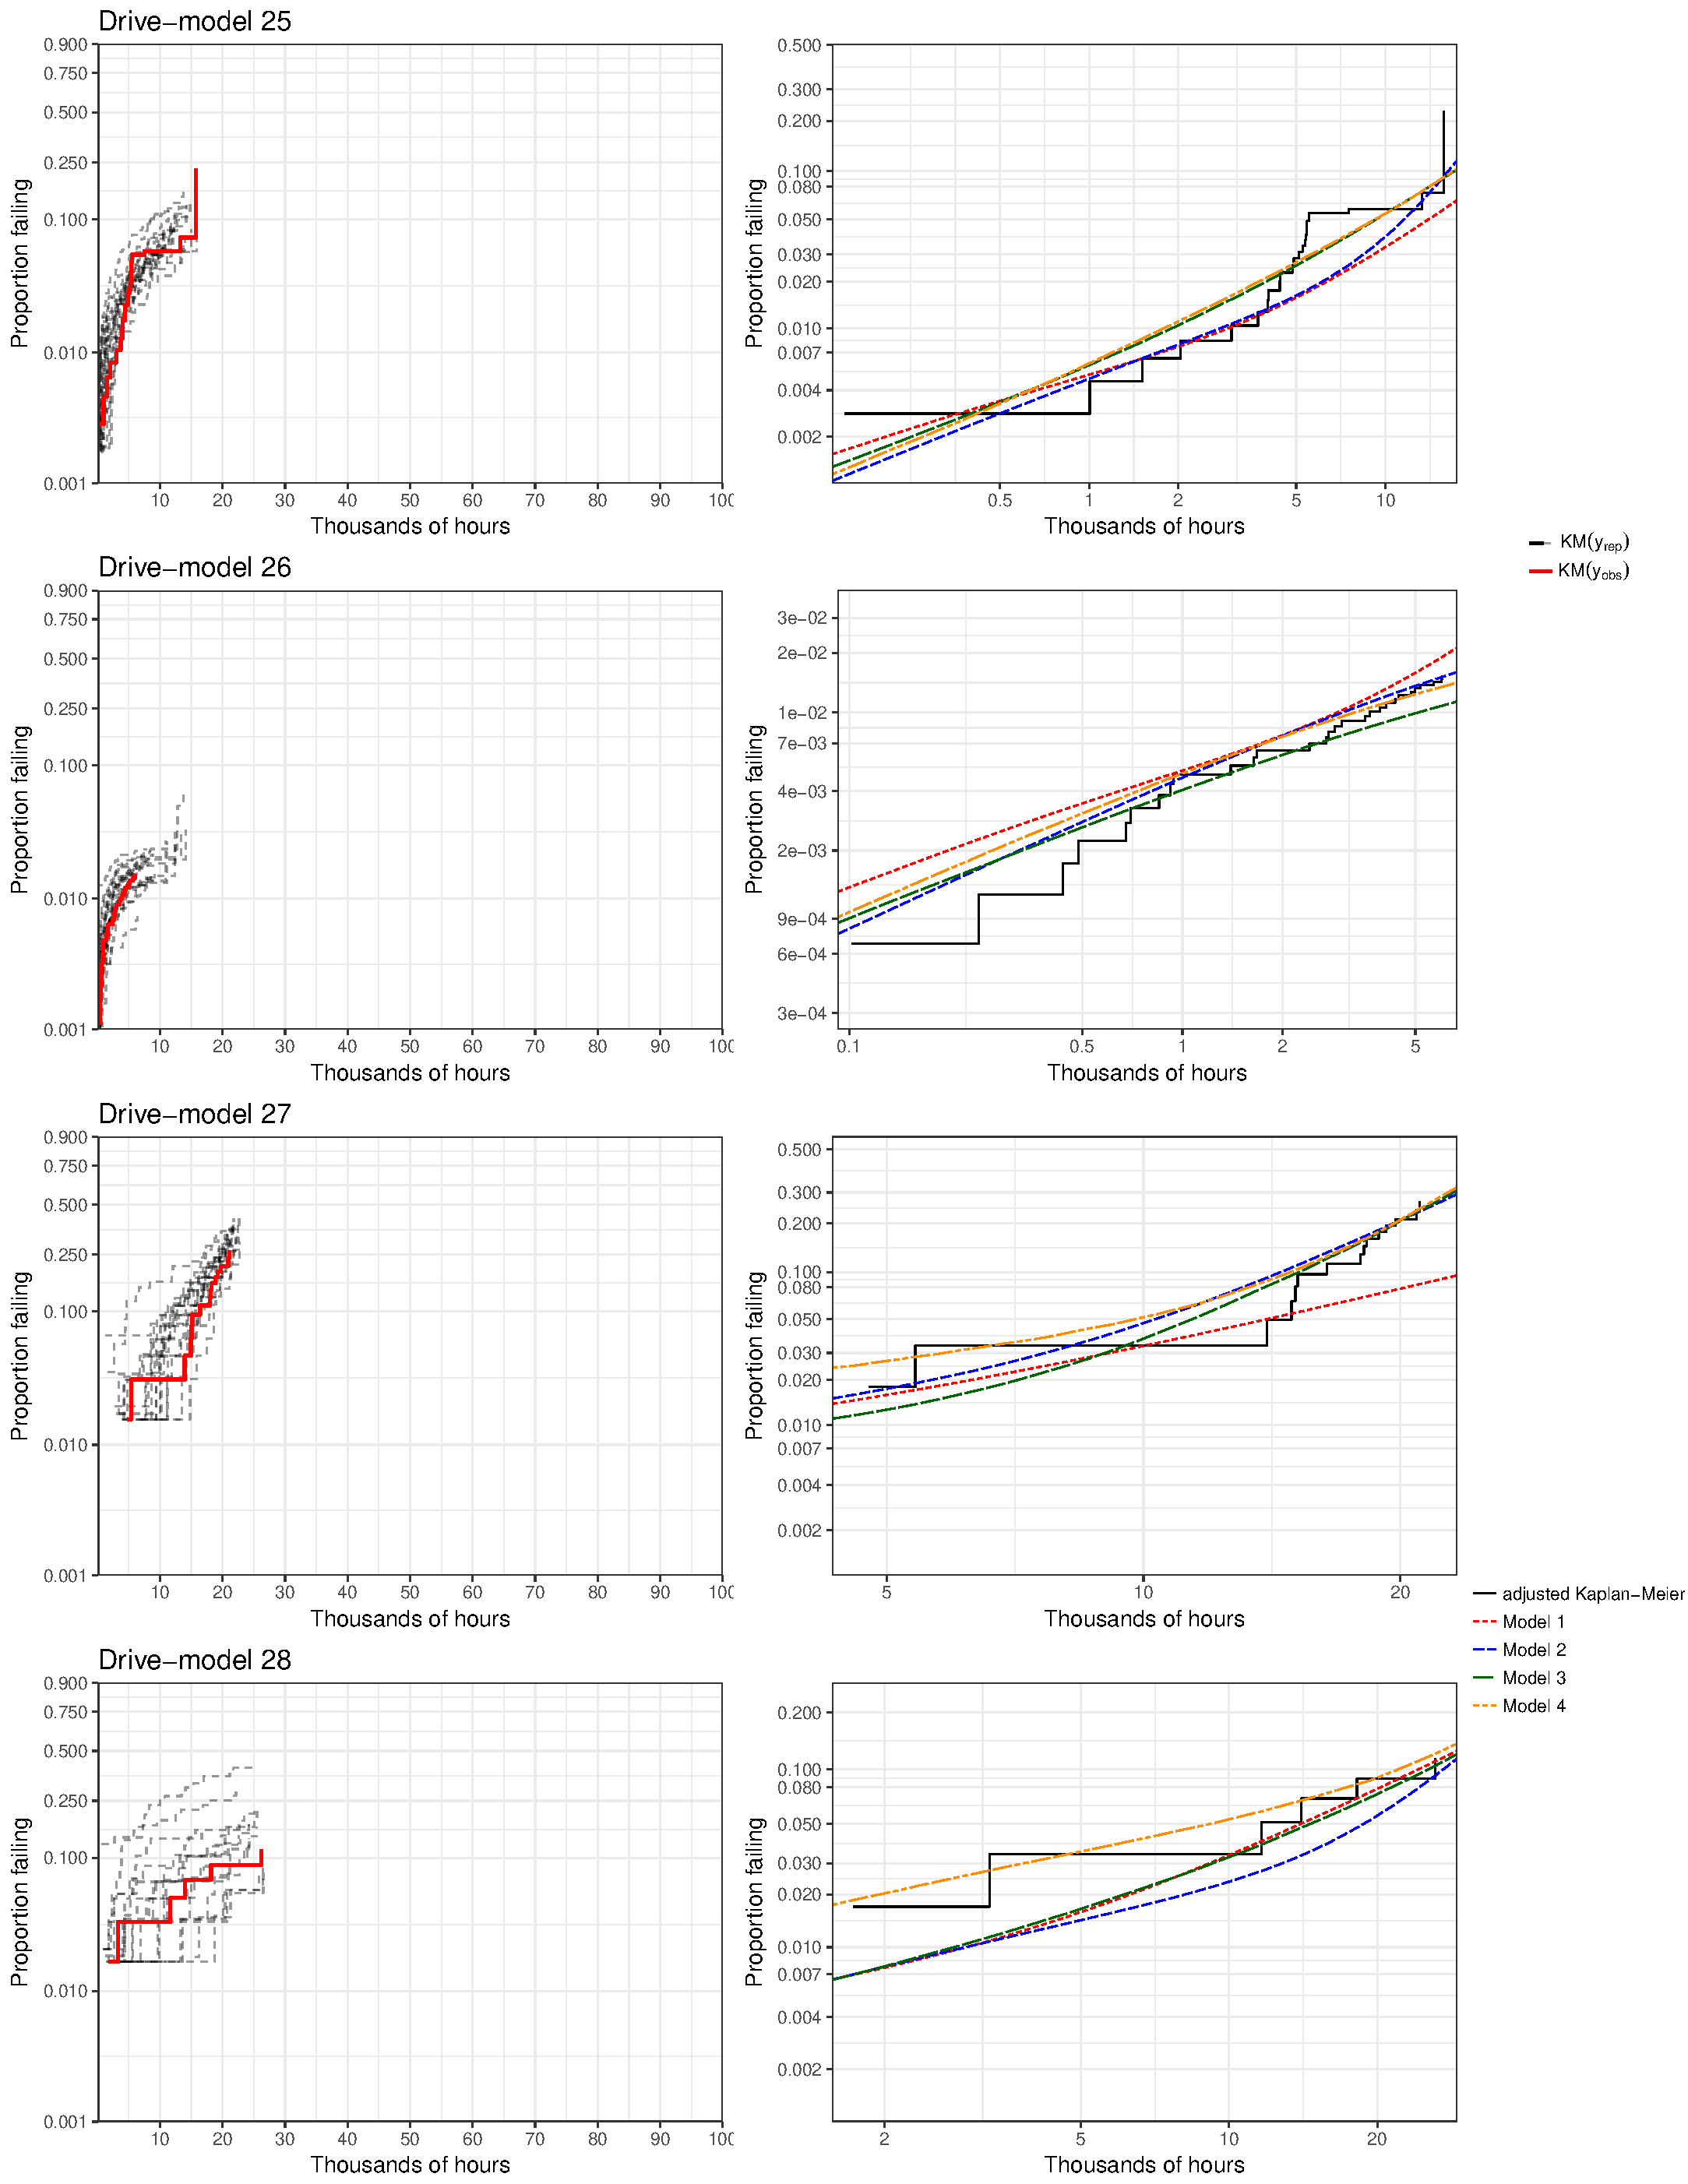
\includegraphics[width=\textwidth]{ppcheck-v3-7.pdf}
\end{figure}
\begin{figure}[H]
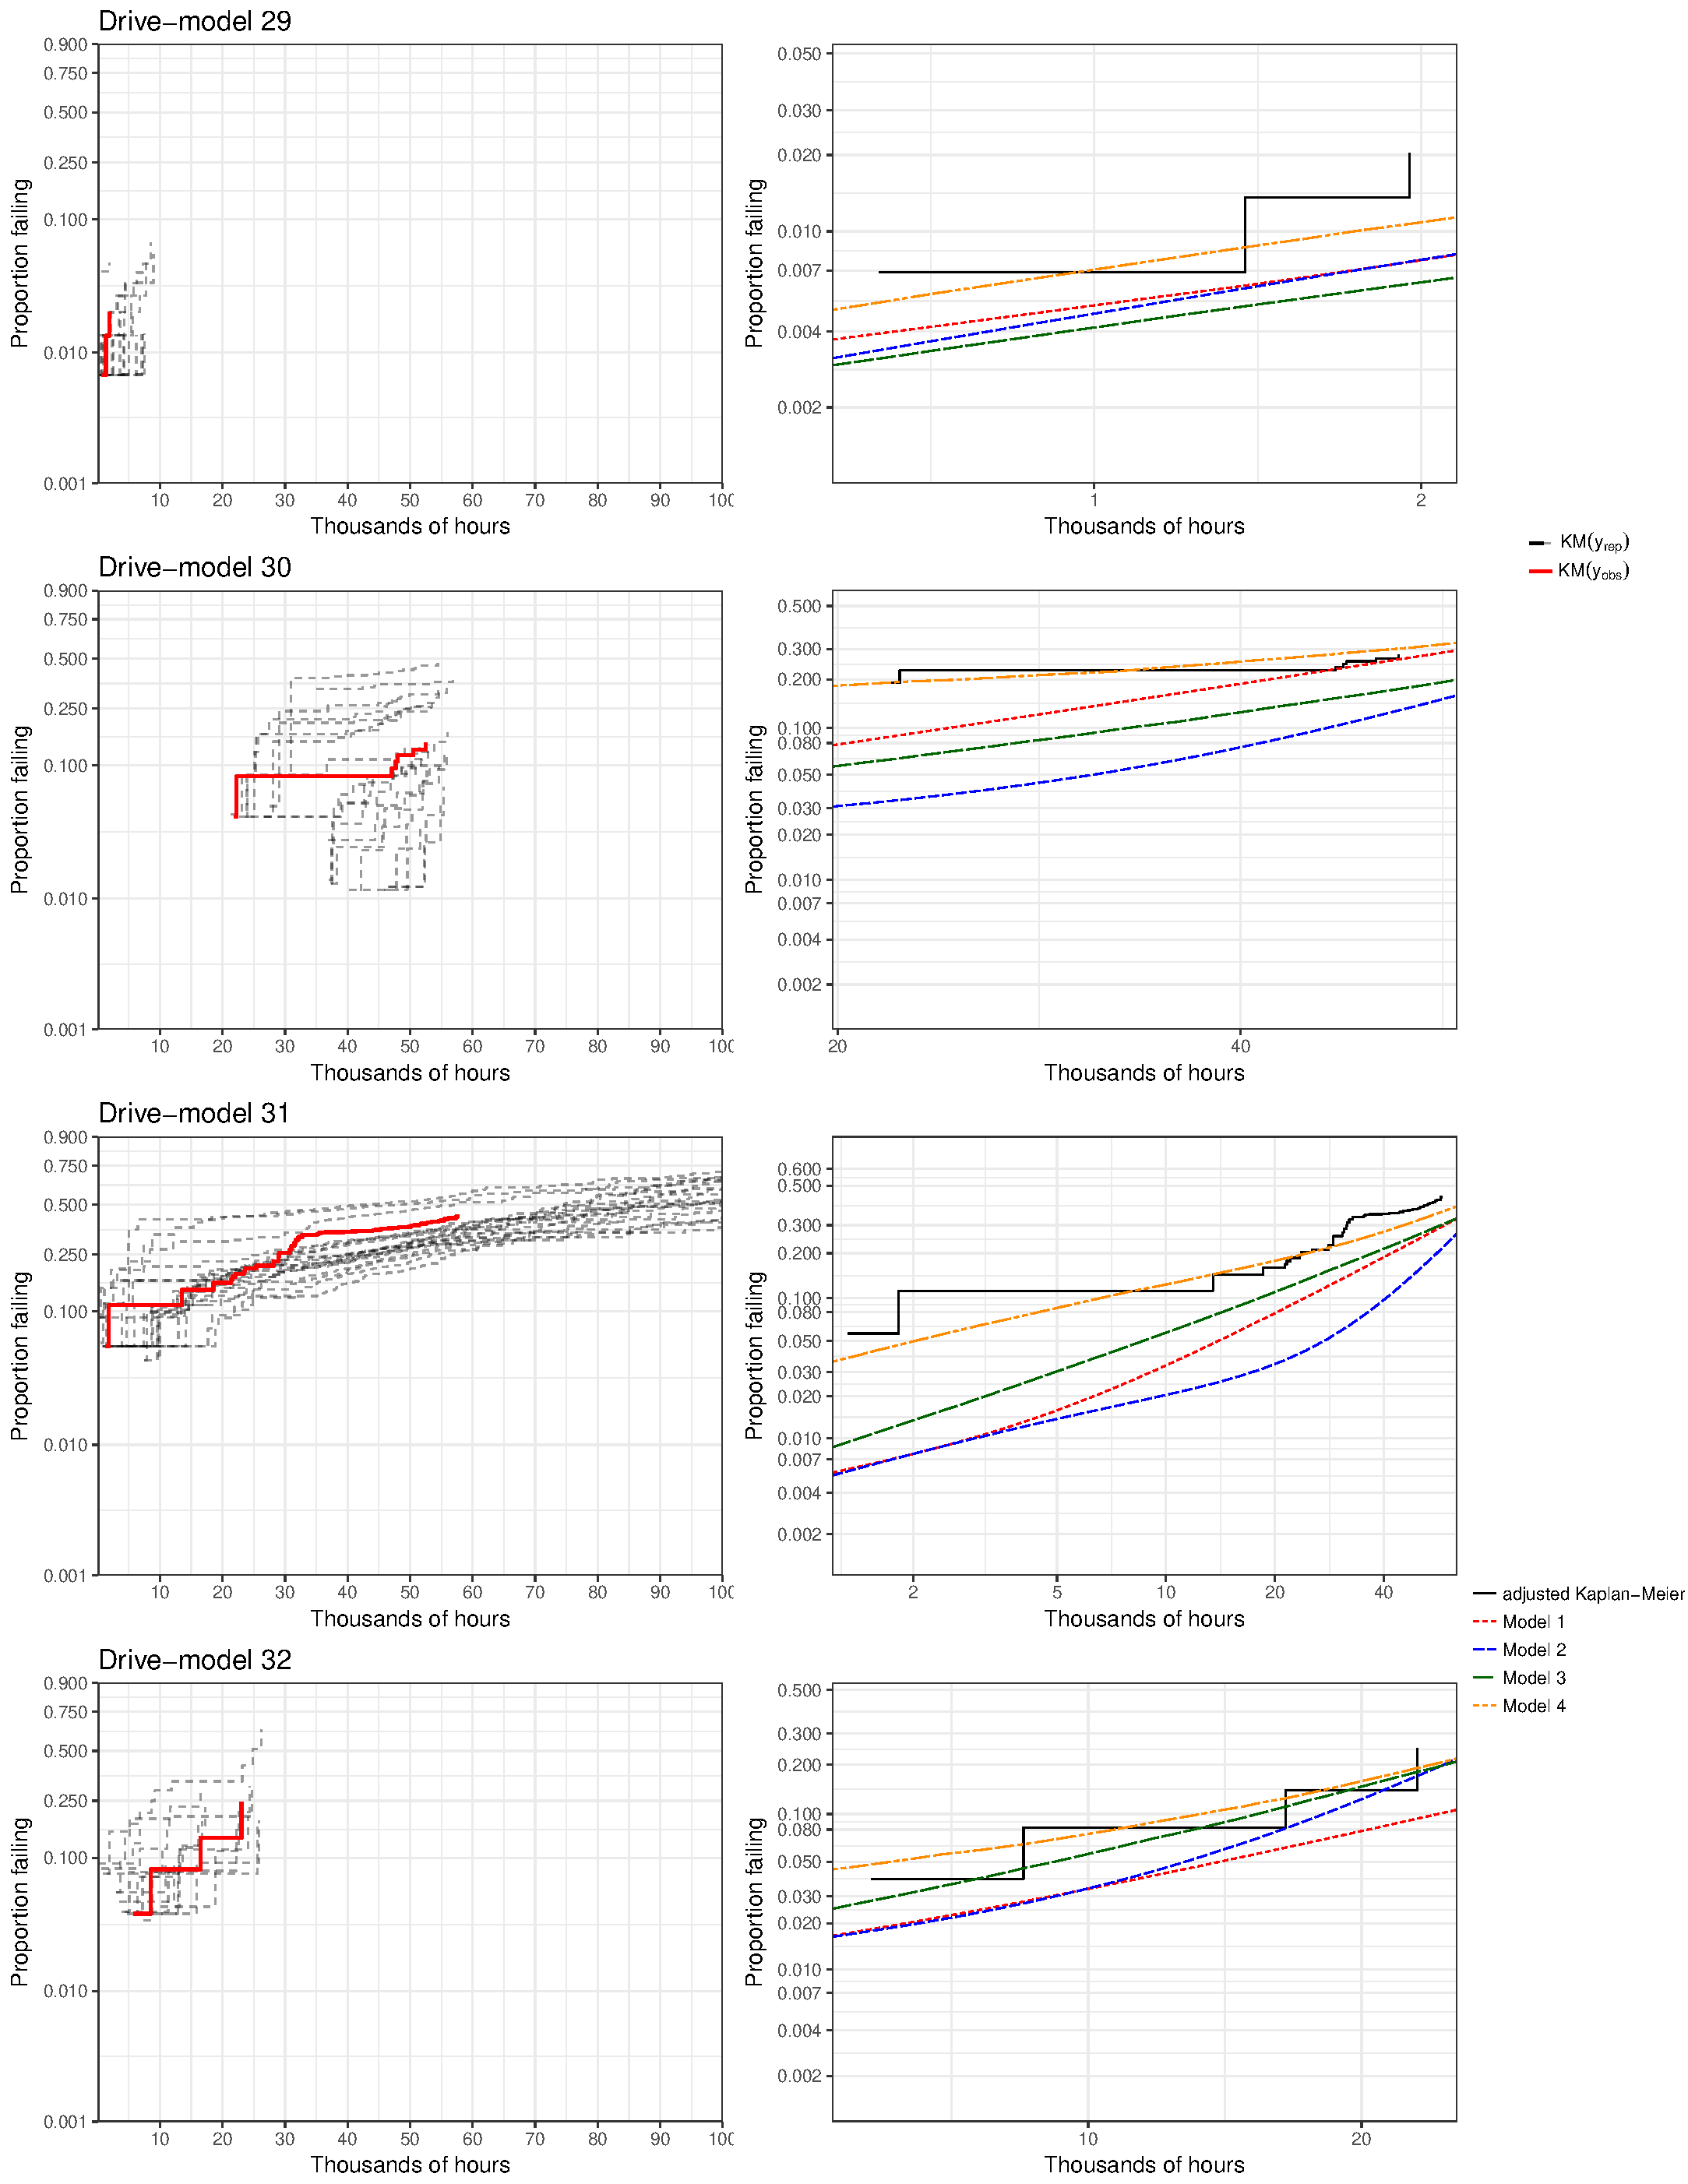
\includegraphics[width=\textwidth]{ppcheck-v3-8.pdf}
\end{figure}
\begin{figure}[H]
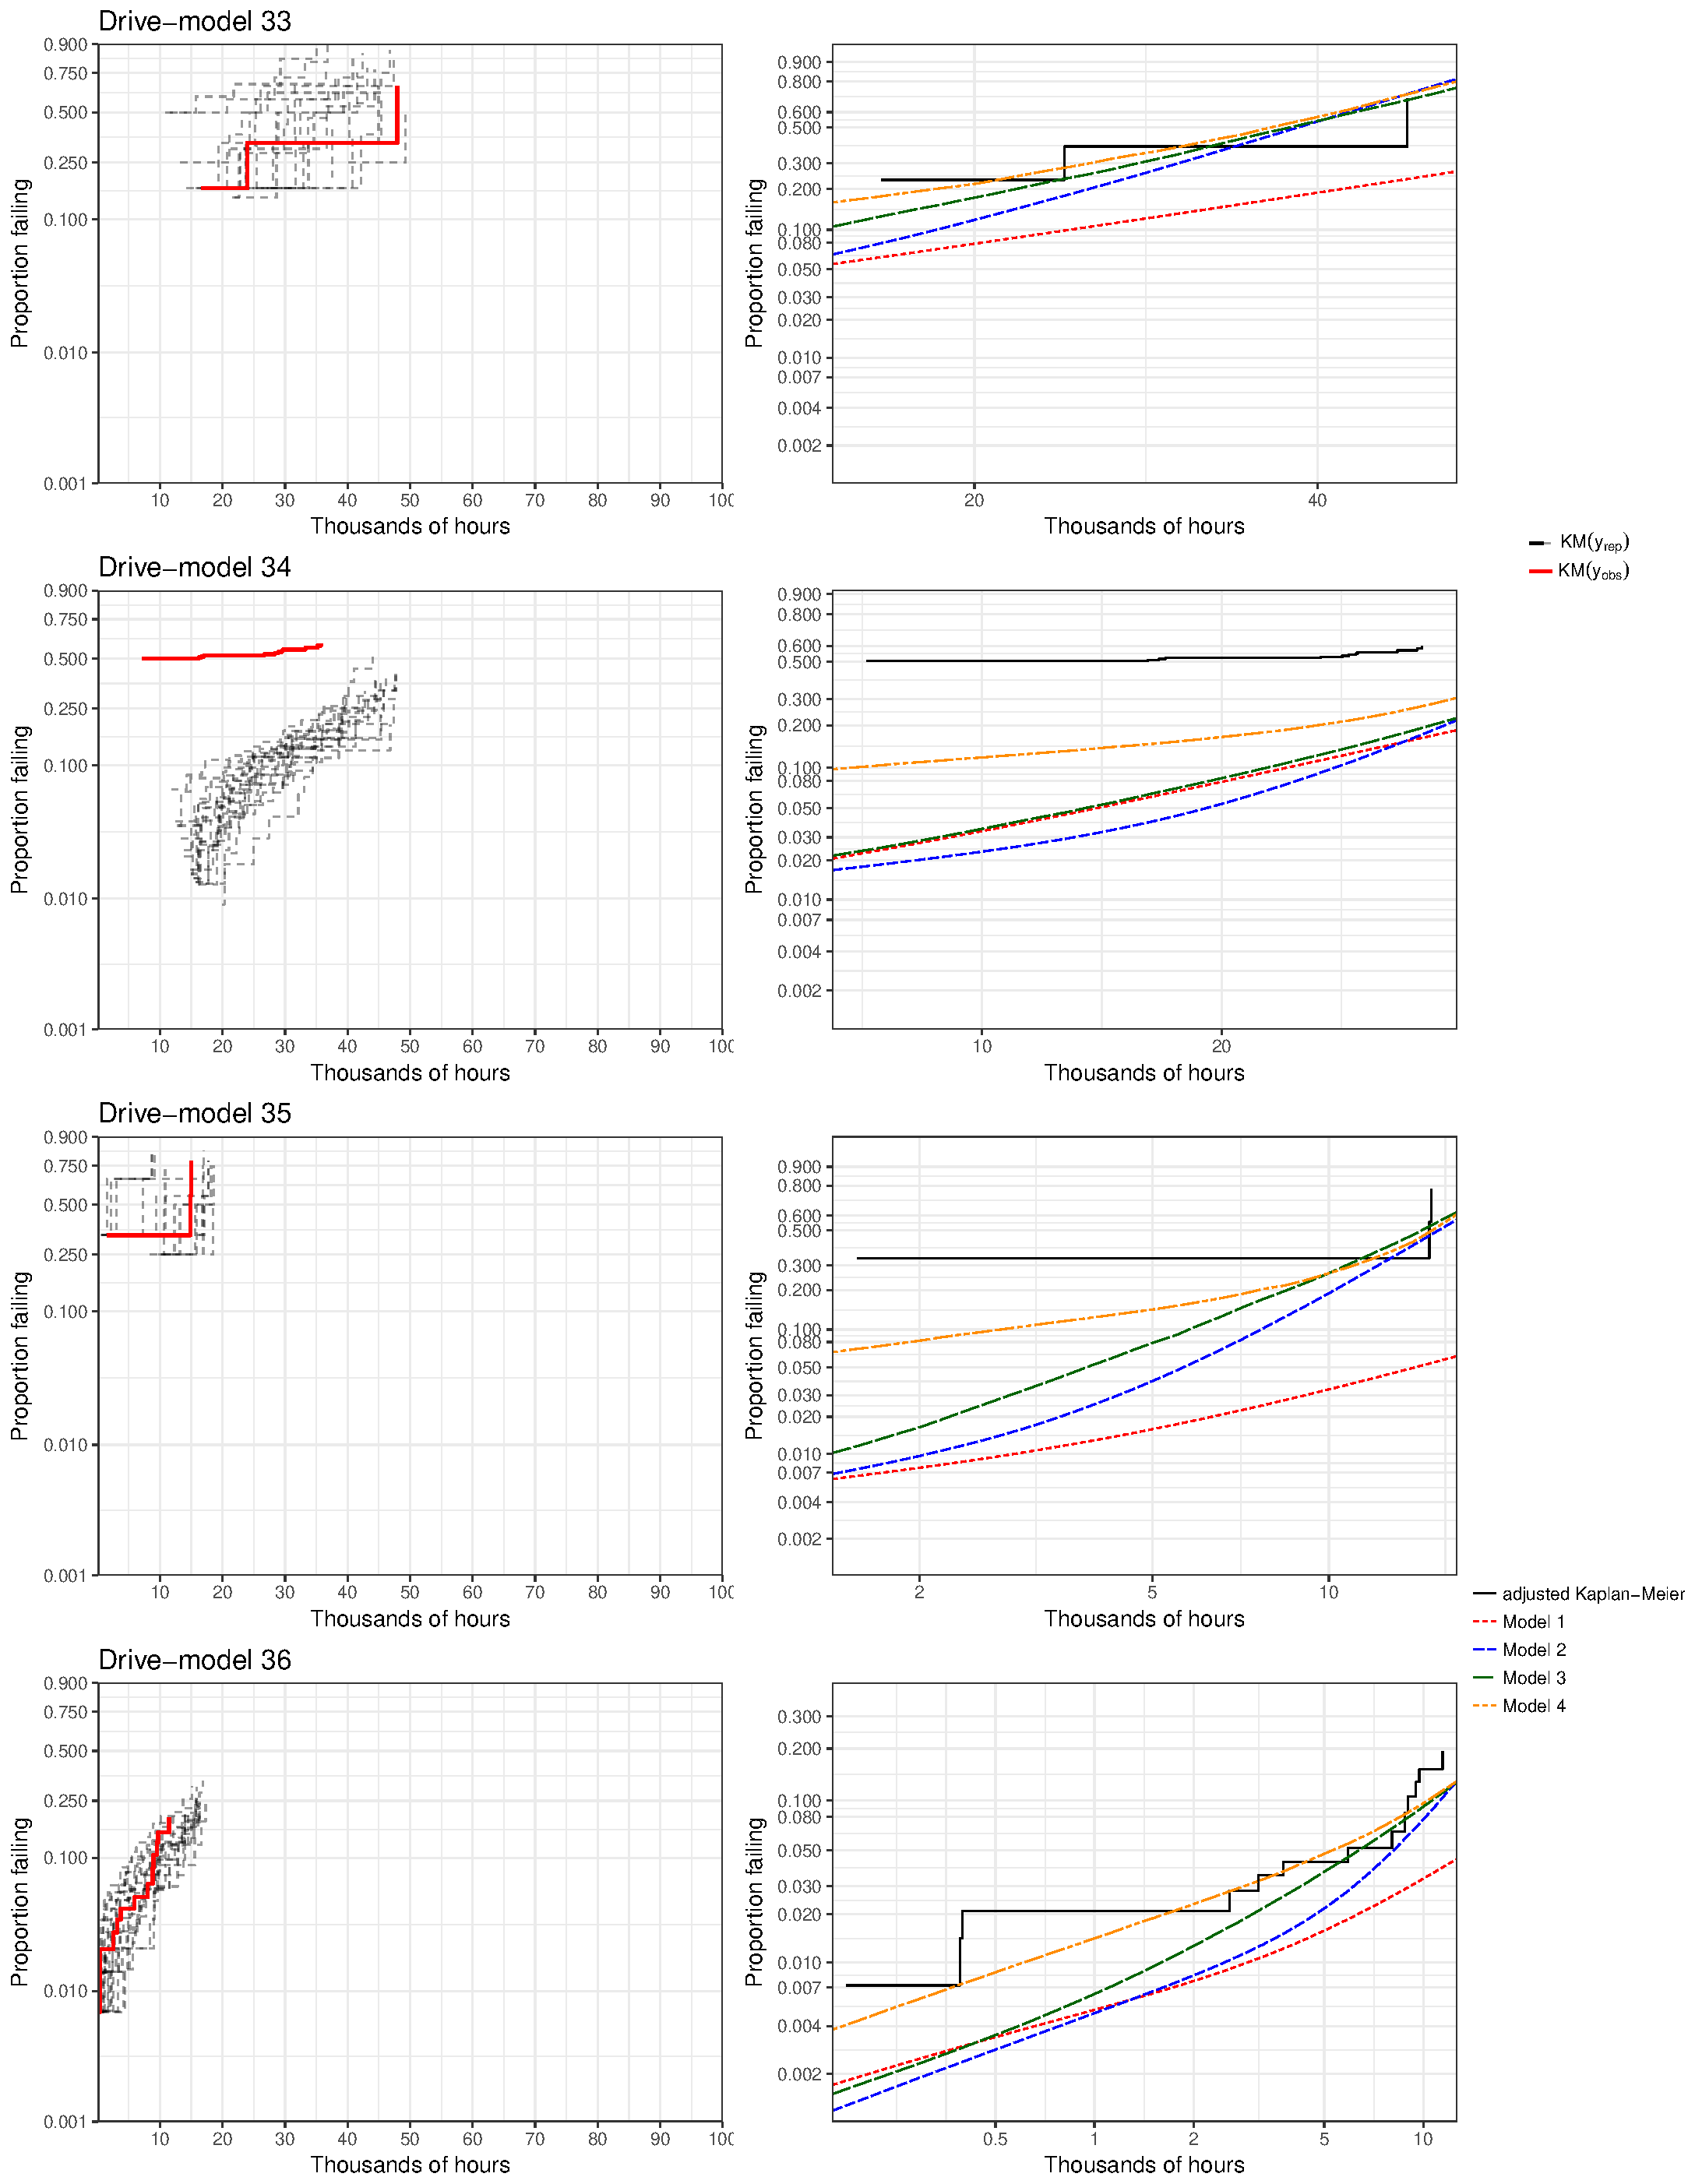
\includegraphics[width=\textwidth]{ppcheck-v3-9.pdf}
\end{figure}
\begin{figure}[H]
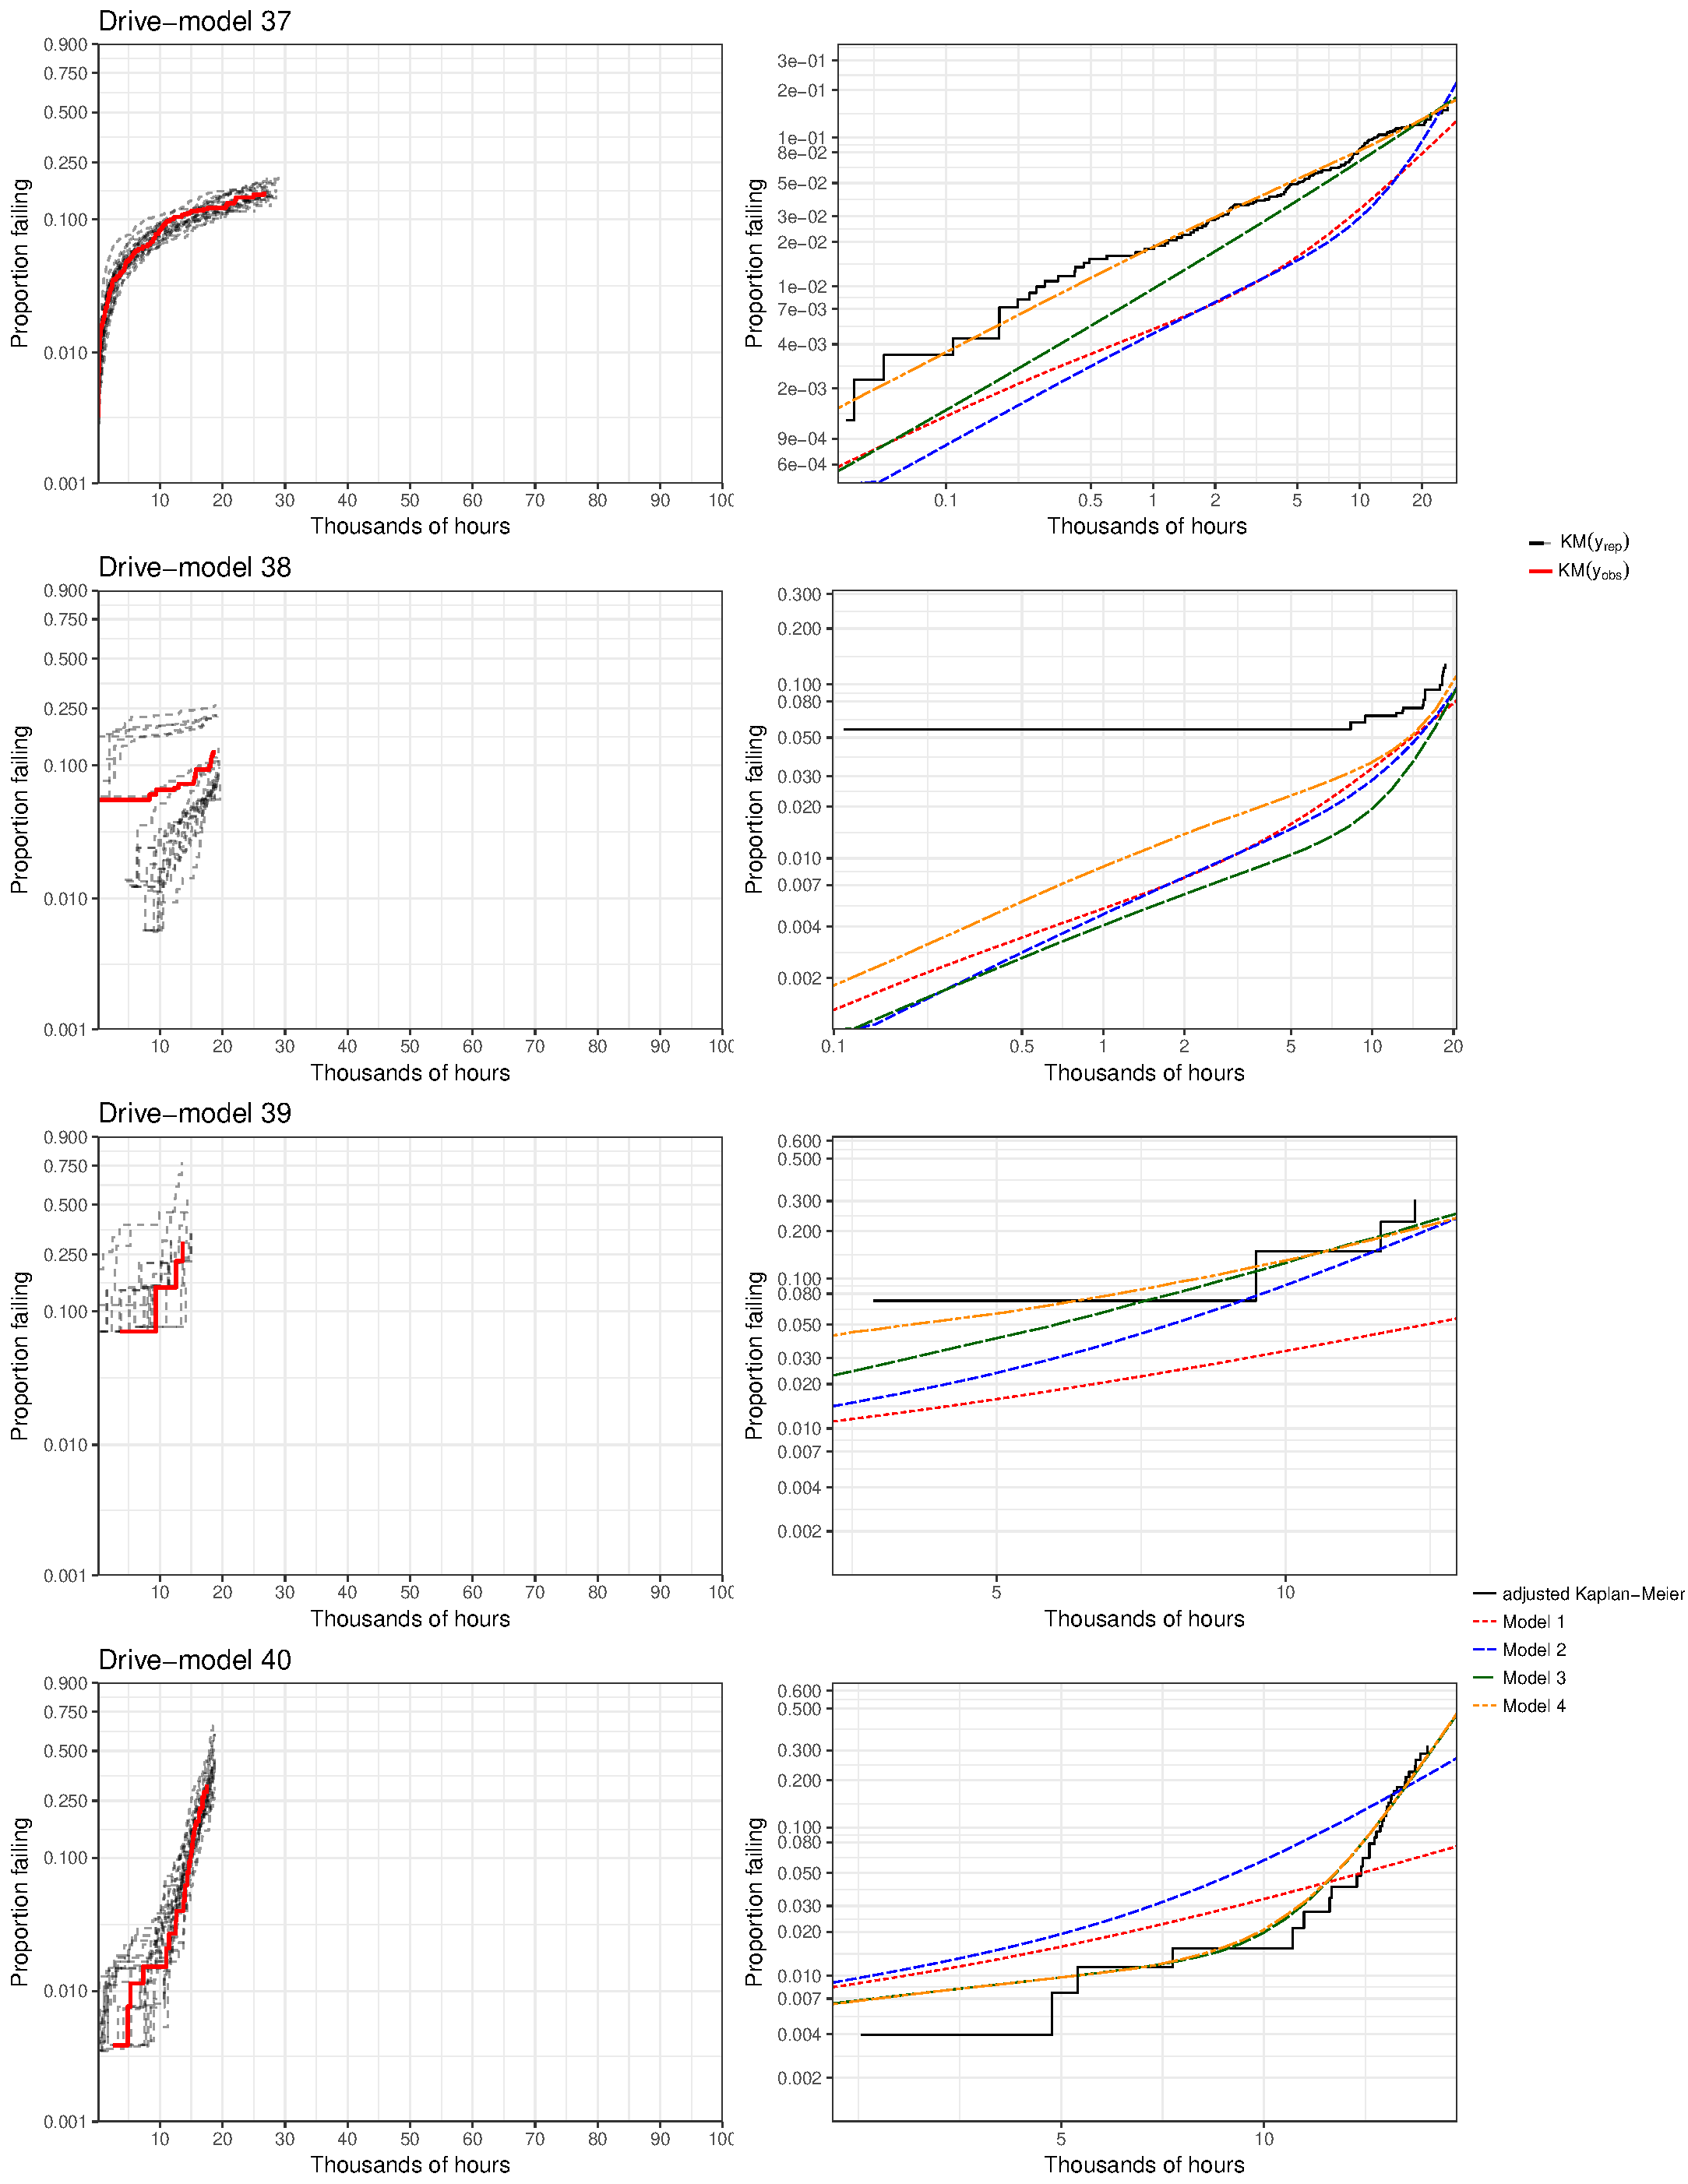
\includegraphics[width=\textwidth]{ppcheck-v3-10.pdf}
\end{figure}
\begin{figure}[H]
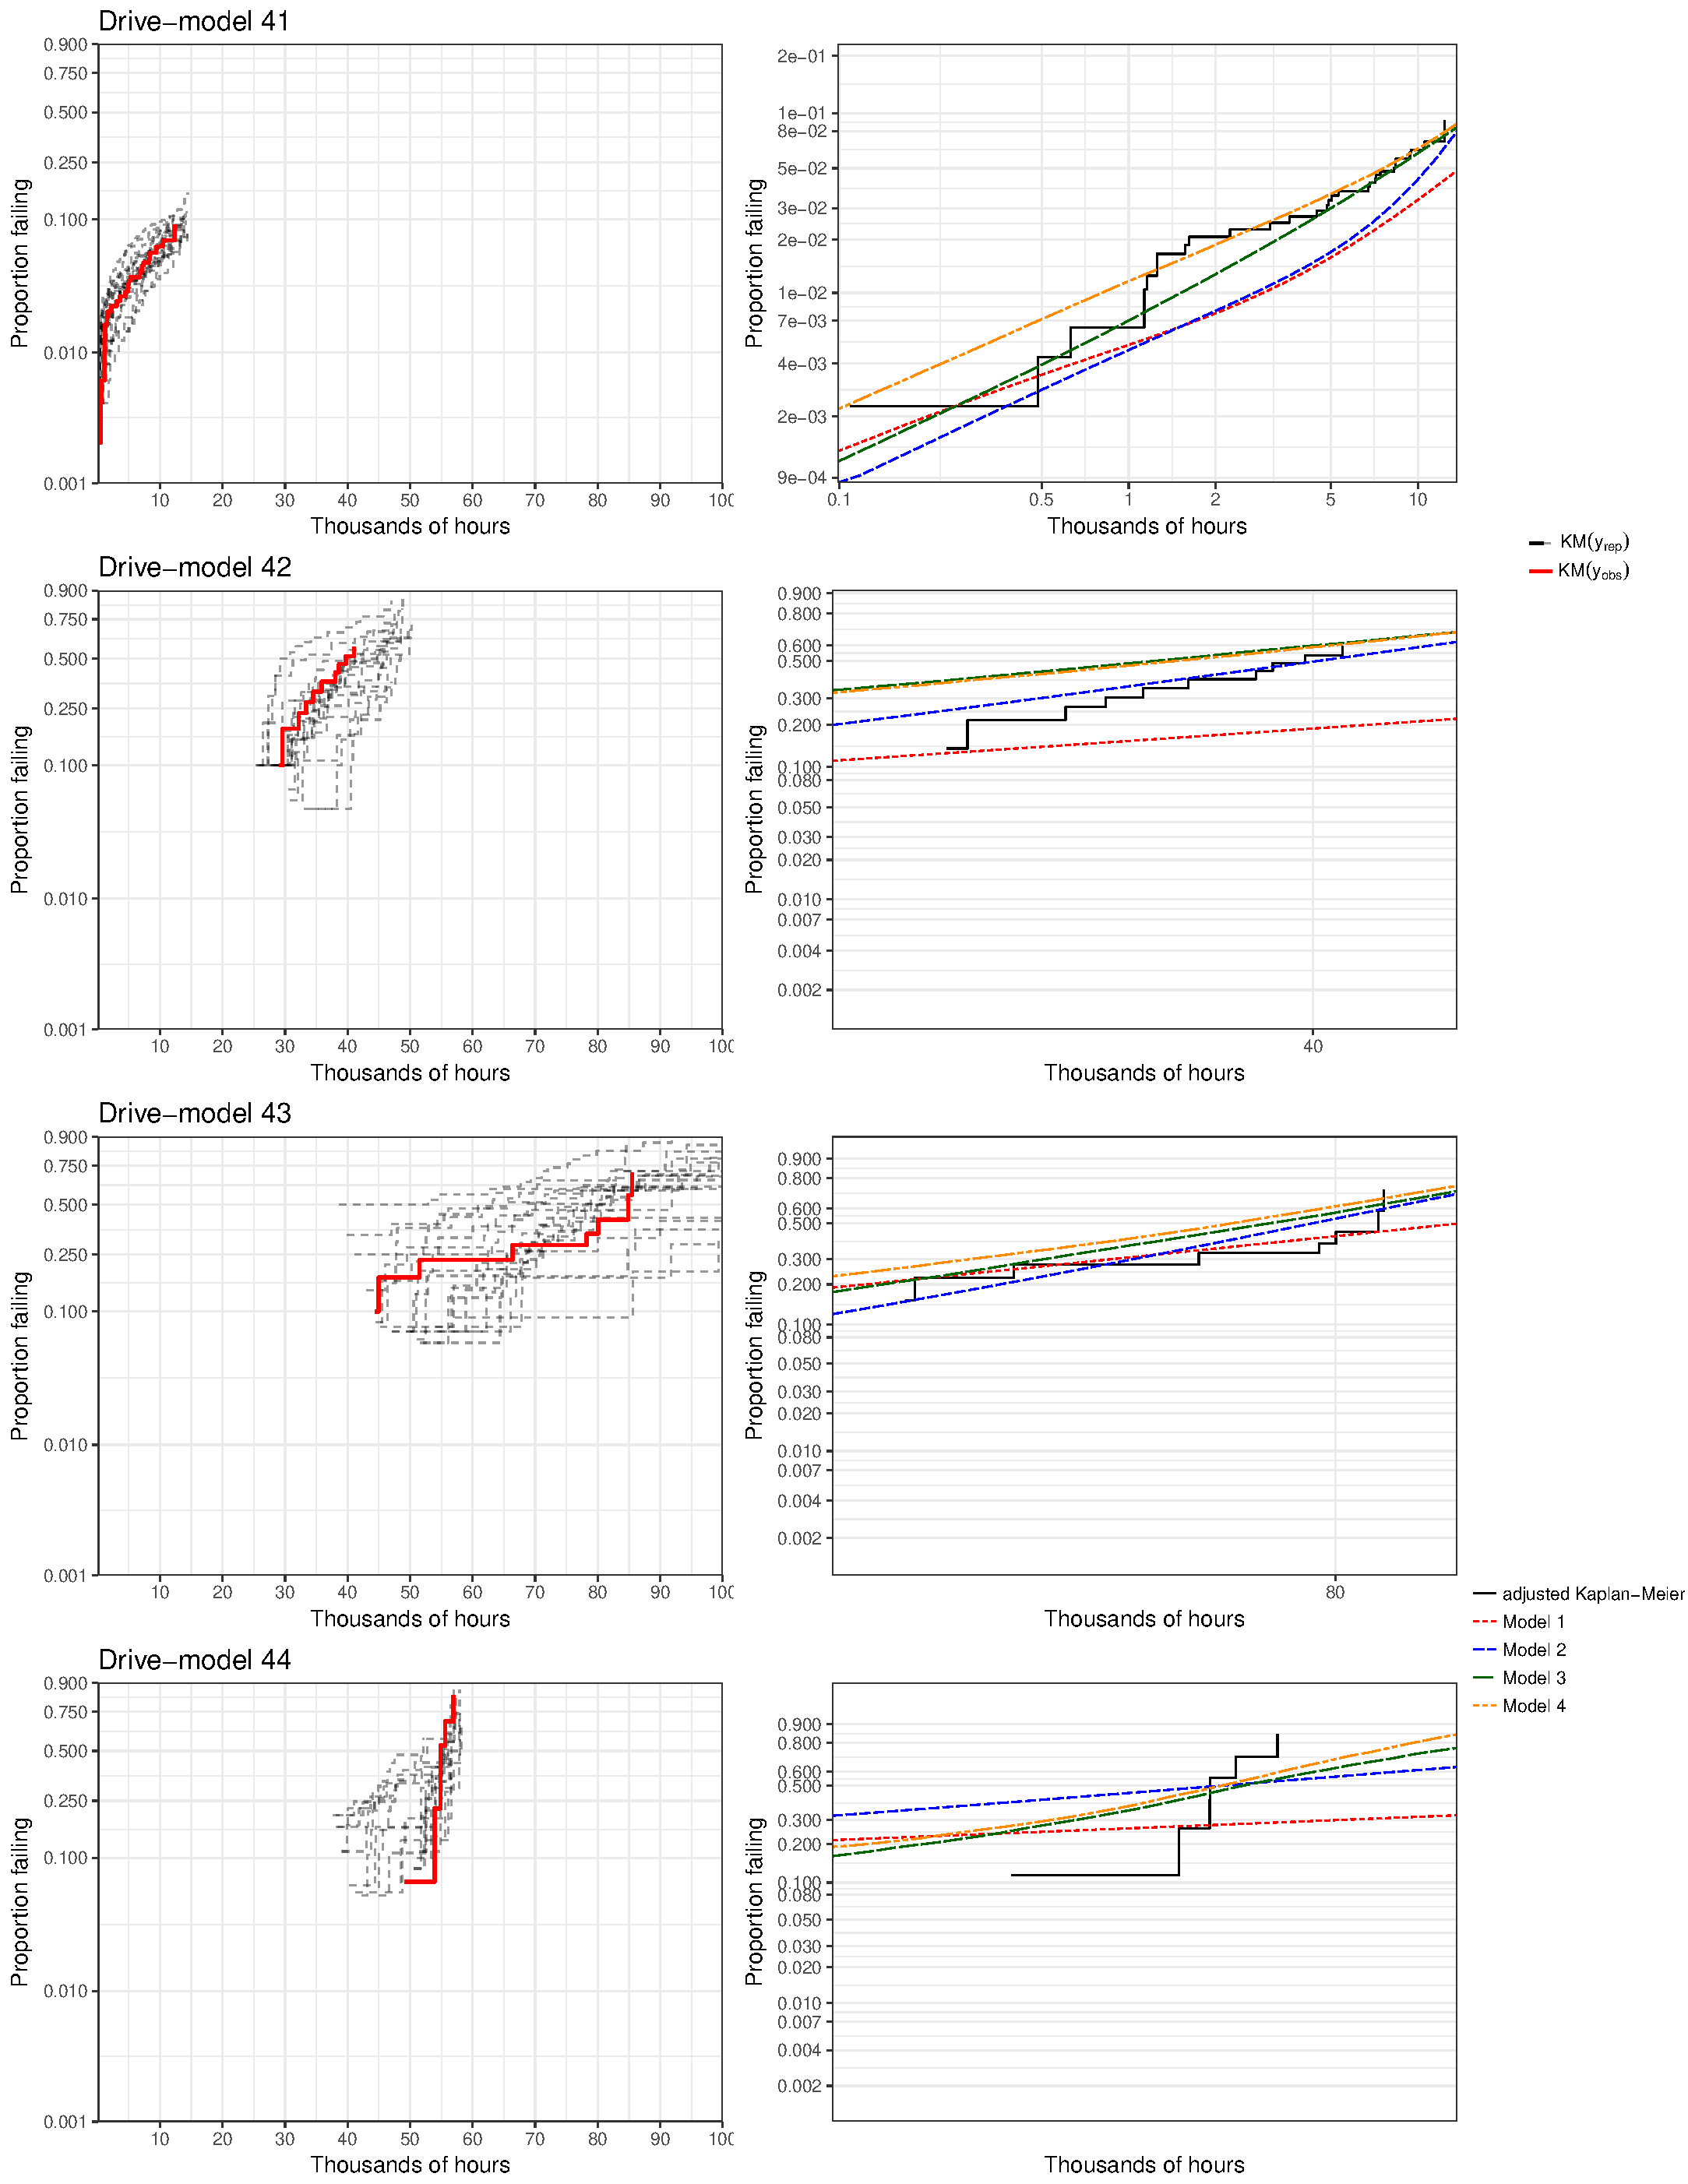
\includegraphics[width=\textwidth]{ppcheck-v3-11.pdf}
\end{figure}
\clearpage


\section{Density Plots for Prior Distributions}
To better visualize the prior distributions, below are plots of
the prior densities for Models 1 - 4.
\begin{figure}[H]
\center
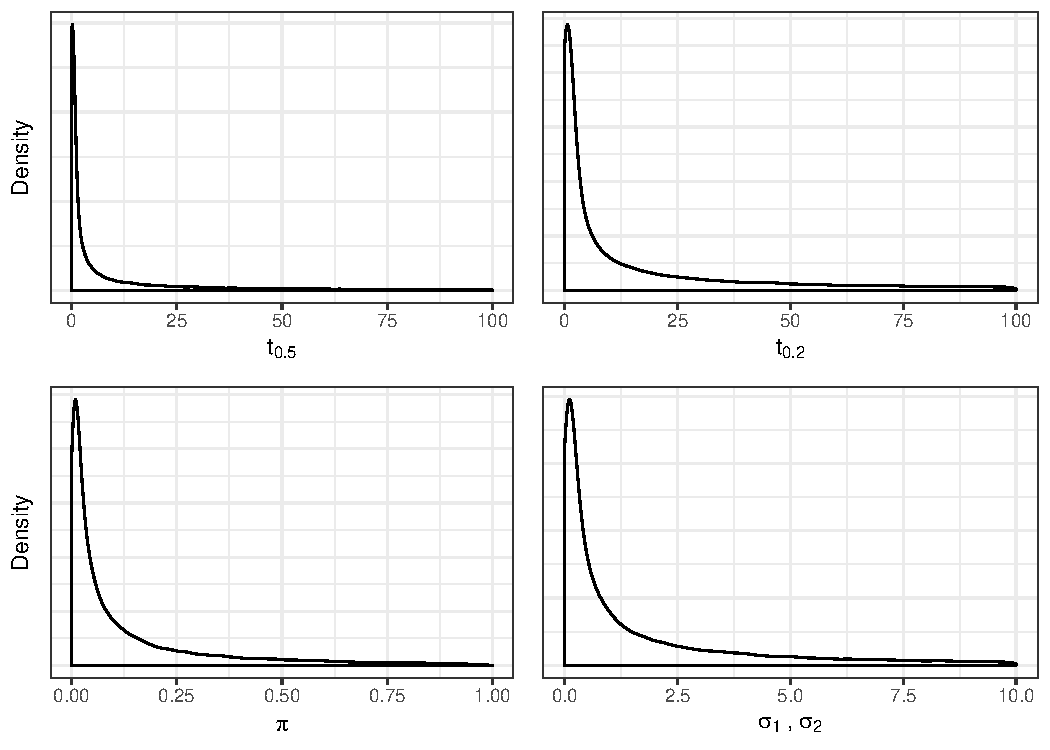
\includegraphics[width=\textwidth]{priorsmod1.pdf}
\caption{Prior Densities for Model 1.  For $t_{p1 = 0.5}$, $t_{p2 = 0.2}$, $x$-axis is in thousands of hours.}
\end{figure}

\begin{figure}[H]
\center
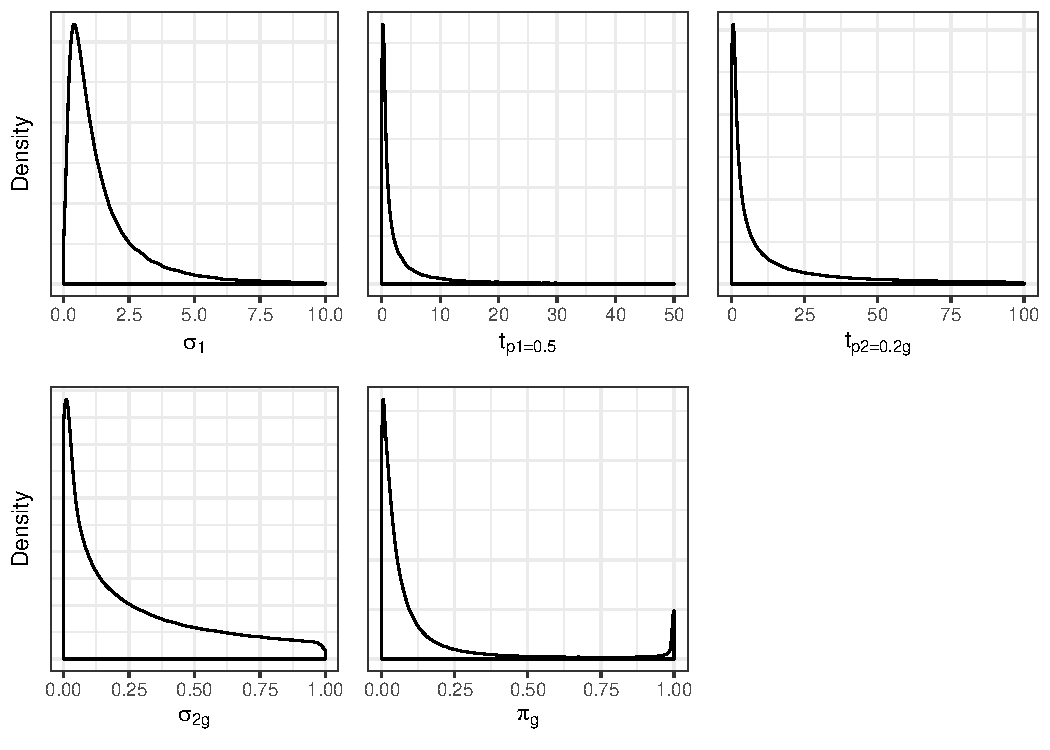
\includegraphics[width=\textwidth]{priormod234.pdf}
\caption{Prior Densities for Models 2 - 4 (top left to bottom right). For $t_{p1 = 0.5}$, $t_{p2 = 0.2g}$, $x$-axis is in thousands of hours.}
\end{figure}

\section{Sensitivity check}
To check whether the posterior distribution of the location hyperparameters, $\eta_\pi$, $\eta_{t_{p_2}}$ and $\eta_{\sigma_2}$ in Model 4 was sensitive to our choice of prior distributions for these parameters, we refit Model 4 doubling the scale of the prior distributions, i.e.
$$\eta_\pi \sim \text{N}(-3,2^2),\; \eta_{t_{p_2}} \sim \text{N}(9,4^2),\; \eta_{\sigma_2} \sim \text{N}(0, 4^2).$$
Figure \ref{double_var} shows that the posterior was nearly identical with the wider prior distributions. This suggests that the posterior is overwhelmingly driven by the information from the data, rather than from the prior (for either choice of prior.)

\begin{figure}[H]
\center
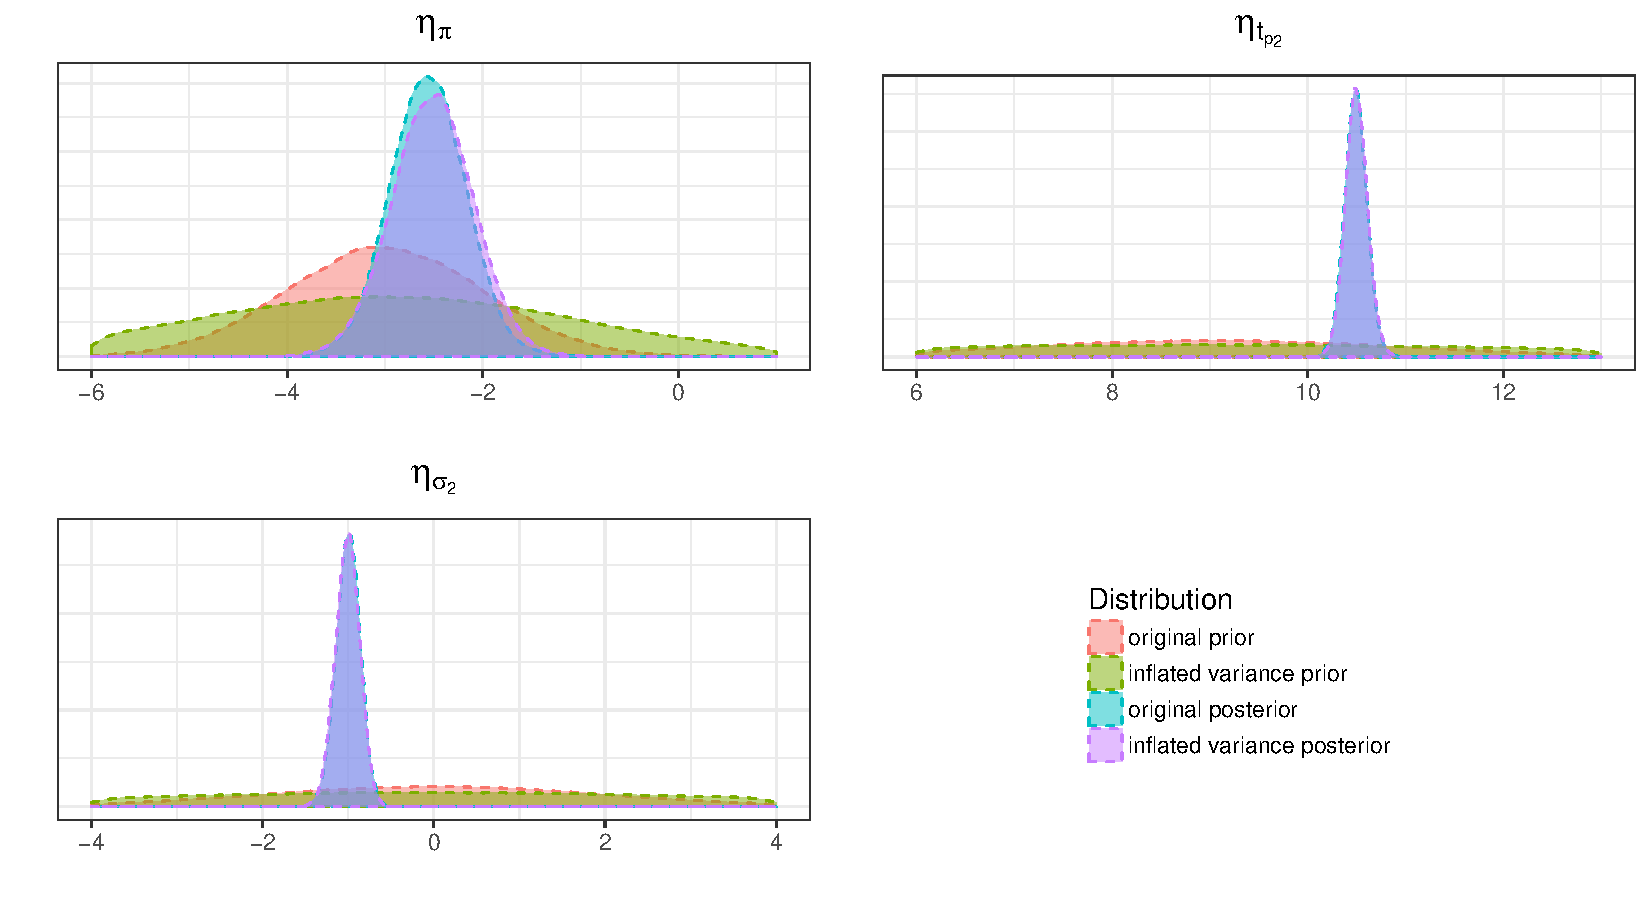
\includegraphics[width=\textwidth]{double_var.pdf}
\caption{Comparison of prior and posterior for location hyperparameters, $\eta_\pi,\; \eta_{t_{p_2}}$ and $\eta_{\sigma_2}$ under the original priors from Section 6.1 and under a modified prior doubling the scale for these parameters.}
\label{double_var}
\end{figure}

\section{Drive Model Brands}
Below are the brand names (provided by Backblaze) corresponding to
the model numbers used in the analysis.
\begin{table}[H]
\centering
\begin{tabular}{lr}
  \hline
Brand Name & Model ID \\ 
  \hline
HGST HDS5C4040ALE630 &   1 \\ 
  HGST HMS5C4040ALE640 &   2 \\ 
  HGST HMS5C4040BLE640 &   3 \\ 
  Hitachi HDS5C3030ALA630 &   4 \\ 
  Hitachi HDS5C4040ALE630 &   5 \\ 
  Hitachi HDS722020ALA330 &   6 \\ 
  Hitachi HDS723020BLA642 &   7 \\ 
  Hitachi HDS723030ALA640 &   8 \\ 
  ST1500DL003 &   9 \\ 
  ST2000DL001 &  10 \\ 
  ST2000DL003 &  11 \\ 
  ST250LM004 HN &  12 \\ 
  ST250LT007 &  13 \\ 
  ST3000DM001 &  14 \\ 
  ST31500341AS &  15 \\ 
  ST31500541AS &  16 \\ 
  ST3160316AS &  17 \\ 
  ST3160318AS &  18 \\ 
  ST32000542AS &  19 \\ 
  ST320005XXXX &  20 \\ 
  ST320LT007 &  21 \\ 
  ST33000651AS &  22 \\ 
  ST4000DM000 &  23 \\ 
  ST4000DX000 &  24 \\ 
  ST500LM012 HN &  25 \\ 
  ST6000DX000 &  26 \\ 
  ST9250315AS &  27 \\ 
  TOSHIBA DT01ACA300 &  28 \\ 
  TOSHIBA MD04ABA400V &  29 \\ 
  WDC WD10EACS &  30 \\ 
  WDC WD10EADS &  31 \\ 
  WDC WD10EADX &  32 \\ 
  WDC WD1600AAJB &  33 \\ 
  WDC WD1600AAJS &  34 \\ 
  WDC WD1600BPVT &  35 \\ 
  WDC WD20EFRX &  36 \\ 
  WDC WD30EFRX &  37 \\ 
  WDC WD30EZRX &  38 \\ 
  WDC WD3200BEKX &  39 \\ 
  WDC WD5000LPVX &  40 \\ 
  WDC WD60EFRX &  41 \\ 
  WDC WD800AAJB &  42 \\ 
  WDC WD800BB &  43 \\ 
  WDC WD800JB &  44 \\ 
   \hline
\end{tabular}
\end{table}

\bibliography{./sample}


\end{document}